% preamble

\documentclass[12pt]{article}

% for special characters
\usepackage[utf8]{inputenc}
\usepackage[T1]{fontenc}
\usepackage{lmodern}
% for images
\usepackage{graphicx}
\graphicspath{{img/}}
% for source in images
\usepackage{floatrow}
% for urls
\usepackage{url}
% for references
\usepackage[sorting=none]{biblatex}
\addbibresource{references.bib}
% for multiple images
\usepackage{subfig}
% for automatic reference prefix
\usepackage{hyperref}
% for uppercase reference at the beginning of a sentence
\usepackage{cleveref}
% for good looking tables
\usepackage{booktabs}
% for lists with a), b), c)
\usepackage{enumitem}
% for equations with multicases
\usepackage{amsmath}
% for float barrier
\usepackage{placeins}

\begin{document}

\title{
\vspace{-2.0cm}

\includegraphics{zhaw}\\ 
\vspace{2cm}
\textbf{Arthritis Net}\\
\vspace{1cm}
\Large Automated bone erosion scoring for rheumatoid arthritis with deep convolutional neural networks\\
\vspace{1cm}
{\Large Zurich University of Applied Sciences}}
\author{\begin{tabular}{rl}
  \textbf{Author:} & Janick Rohrbach \\
  \textbf{Supervisor:} & Prof. Dr. Oliver Dürr \\ & Prof. Dr. Beate Sick \\
  \textbf{Industrial Partner:} & Seantis GmbH \\
  \textbf{External Supervisor:} & Fabian Reinhard \\ & Dr. Tobias Reinhard \\
  \textbf{Date:} & December 22, 2017 \\
  \hspace{6.0cm} & \hspace{6.0cm}
\end{tabular}}
\date{}
\maketitle

\newpage

\section*{Declaration of originality\\ \large{Project Thesis at the School of Engineering}}
By submitting this project thesis, the undersigned student confirms that this thesis is his own work and was written without the help of a third party. \\
\\
The student declares that all sources in the text (including Internet pages) and appendices have been correctly disclosed. This means that there has been no plagiarism, i.e. no sections of the project thesis have been partially or wholly taken from other texts and represented as the student’s own work or included without being correctly referenced. \\
\\
Any misconduct will be dealt with according to paragraphs 39 and 40 of the General Academic Regulations for Bachelor’s and Master’s Degree courses at the Zurich University of Applied Sciences (Rahmenprüfungsordnung ZHAW (RPO)) and subject to the provisions for disciplinary action stipulated in the University regulations.\\
\vspace{3cm} \\
Zurich, December 22, 2017 \hspace{5cm} Janick Rohrbach

\newpage

\section*{Abstract}

Rheumatoid arthritis can cause irreversible damage to the joints. The severity of those bone erosions is scored by using x-ray images. This is usually done by a trained rheumatologist or radiologist and takes several minutes per patient.

This thesis shows a method to automatically score the joints in x-ray images with deep convolutional neural networks. We take a classification and a regression approach on x-ray images of joints from the left hand. In the classification task we predict the Ratingen-score on a discrete integer scale from 0 to 5. The model achieves class normalized validation and test accuracies of 42 \% and 43 \% respectively. The class normalized accuracies for predictions that are off by no more than 1 class are 82 \% for the validation set and 83 \% for the test set. The regression model predicts the continuous percentage of bone erosion between 0 \% and 100 \% with a validation and test mean squared error of 72.8 and 97.6 respectively. The mean absolute error is 3.1 for the validation set and 3.5 for the test set.

An automated scoring of bone erosion could help rheumatologists to spend less time with the scoring and have more time with the patient.

\newpage

\section*{Acknowledgements}
I would like to express my sincere thanks to my supervisors Oliver Dürr and Beate Sick who provided me with guidance and support during the writing of this thesis. 

I would also like to thank Fabian Reinhard and Tobias Reinhard (Seantis GmbH) for their valuable inputs. 

Further, I want to acknowledge the SCQM foundation which made this thesis possible by providing the comprehensive dataset. A list of rheumatology offices and hospitals that are contributing to the SCQM registries can be found on www.scqm.ch/institutions. The SCQM is financially supported by pharmaceutical industries and donors. A list of financial supporters can be found on www.scqm.ch/sponsors.

\newpage

\tableofcontents

\newpage

\section{Introduction}

This thesis shows an automated method with deep convolutional neural networks for the scoring of x-ray images of patients with rheumatoid arthritis. The main task of the scoring is to measure the destruction of the joint. \cite{rau_2007} We show a classification model that predicts the Ratingen-score and a regression model which predicts the percentage of bone erosion. Existing works such as the article by Sharp et al. \cite{sharp_2000} or the article by Ichikawa et al.\cite{ichikawa_2017} semi-automate the joint space measurement of finger joints. Sharp et al. further show a method to estimate the bone erosion from the joint space measurement. In contrast to those existing works, our method is fully automated and directly scores the bone erosion.

\subsection{Background}

Rheumatoid arthritis is an autoimmune disease, which means that the disease is caused by a malfunctioning immune system. The immune system attacks healthy tissue instead of bacteria and viruses. This causes inflammation in the joints. Irreversible damage to the bone in the joint can occur, if the inflammation lasts for a long time. \cite{rheuma} Rheumatoid arthritis is incurable, merely the symptoms can be treated.

Today, the severity of the bone erosion is assessed by a trained rheumatologist by using x-ray images of hand and feet. This process takes several minutes per patient. This thesis shows, how recent advances in computer vision make it possible to automate this task. This leads to time savings which in return help the rheumatologist to spend more time with the patient.

The Swiss Clinical Quality Management in Rheumatic Diseases (SCQM) Foundation runs a national registry of inflammatory rheumatic diseases. \cite{scqm_about} They have collected anonymized patient data for over 10 years and provide the x-ray images used for this analysis.

Seantis GmbH, the industrial partner for this thesis, is a Swiss company that develops data driven web applications for medical research, pubic administration and aviation. \cite{seantis_about} For their customer SCQM they want to automate the bone erosion assessment. They already have a working algorithm, which detects the body part shown in the x-ray image. A second algorithm detects the joints in the image and extracts them as single images. These images are then used together with the bone erosion scores to train our model.

% Stand der Technik: Bisherige Lösungen des Problems und deren Grenzen 
% (Nennt kurz den Industriepartner und/oder weitere Kooperationspartner und dessen/deren Interesse am Thema Fragestellung) 

\subsection{Related literature}

% Nennt bestehende Arbeiten/Literatur zum Thema Literaturrecherche

There are several applications where convolutional neural networks are used in medical research.

An approach similar to ours was presented by a team from the University of California, San Francisco at the Society for Imaging Informatics in Medicine's Conference on Machine Intelligence in Medical Imaging (C-MIMI 2017)\cite{auntminnie}. Norman et al. \cite{norman} trained a deep convolutional neural network on MRI images of the knee joint to extract cartilage volume and thickness measurements. These measurements are used to assess osteoarthritis. This fully automated method drastically reduces the time for an assessment from up to three hours to less than 10 seconds.

A recent paper from Tajbakhsh et al. \cite{tajbakhsh_2017} investigated whether fine-tuning a pre-trained CNN is better than training a CNN from scratch when applied to medical images. They find that pre-trained networks with fine-tuning always outperformed or at least performed as well as CNNs trained from scratch. They further recommend a layer-wise fine tuning which seems to outperform shallow and deep tuning.

A study by Paul et al. \cite{paul_2017} tried to classify osteoporosis by considering x-ray images of the bone. This task proved to be very difficult as the x-ray images from healthy patients look very similar to the ones of patients with the disease. By using a transfer learning approach they achieved a validation accuracy of 44.82 \%.

Zhou et al. \cite{zhou_2002} used a two-level ensemble of neural networks to identify lung cancer cells on x-ray images of the chest. The first-level ensemble classifies whether a cell is a cancer cell or not by using full voting. The second-level ensemble is used only on cells classified by the first-level as cancer cells. It differentiates between different cancer classes as well as a non-cancer class. The ensemble works with plurality voting. The authors state that this method achieves a high accuracy and a low rate of false negatives.

A report from Chen \cite{chen_2016} showed the application of convolutional neural networks on x-ray images of hands to predict the developmental bone age. He achieves a top one and two accuracy of 46 \% and 70 \% respectively. This result is close to previously used methods which use manual segmentation and handcrafted features.

In a degree project Hensman and Masko \cite{hensman_2015} looked at the impact of imbalanced training data for CNNs. They find, that heavy imbalances have a strong impact on the performance and suggest oversampling of minority classes to improve the performance of the network.

\subsection{Aim and scope of this thesis}

The aim of this thesis is to predict bone erosion scores from x-ray images. We further examine how the bone erosion and the disease activity are correlated.

The work is based on images of the left hand only. There also exist images of right hands as well as images of left and right feet. But at this point in time, only the joints of left hands have been extracted from the images. It is assumed that the model will perform similar on the joints of the right hand. By fine-tuning the model on the images of joints from feet it is expected that the model can also be used for those images.

\newpage

\section{Theory}
\label{sec:theory}
This section introduces terms and concepts which greatly help to understand the following sections.

\subsection{Finger joints}
\label{subsec:joints}

\autoref{fig:joints} shows an x-ray image of a left hand similar to the images received from the SCQM foundation. The five proximal interphalangeal (PIP) joints and the five carpometacarpal (MCP) joints are shown with blue bounding boxes. These are the joints, that are most affected by rheumatoid arthritis. The wrist joint is also affected, but we limited our analysis to the five PIP joints and the five MCP joints. Each of these joints is assessed with a score by a trained rheumatologist or radiologist. The scoring method is described in the next section.

\begin{figure}[ht]
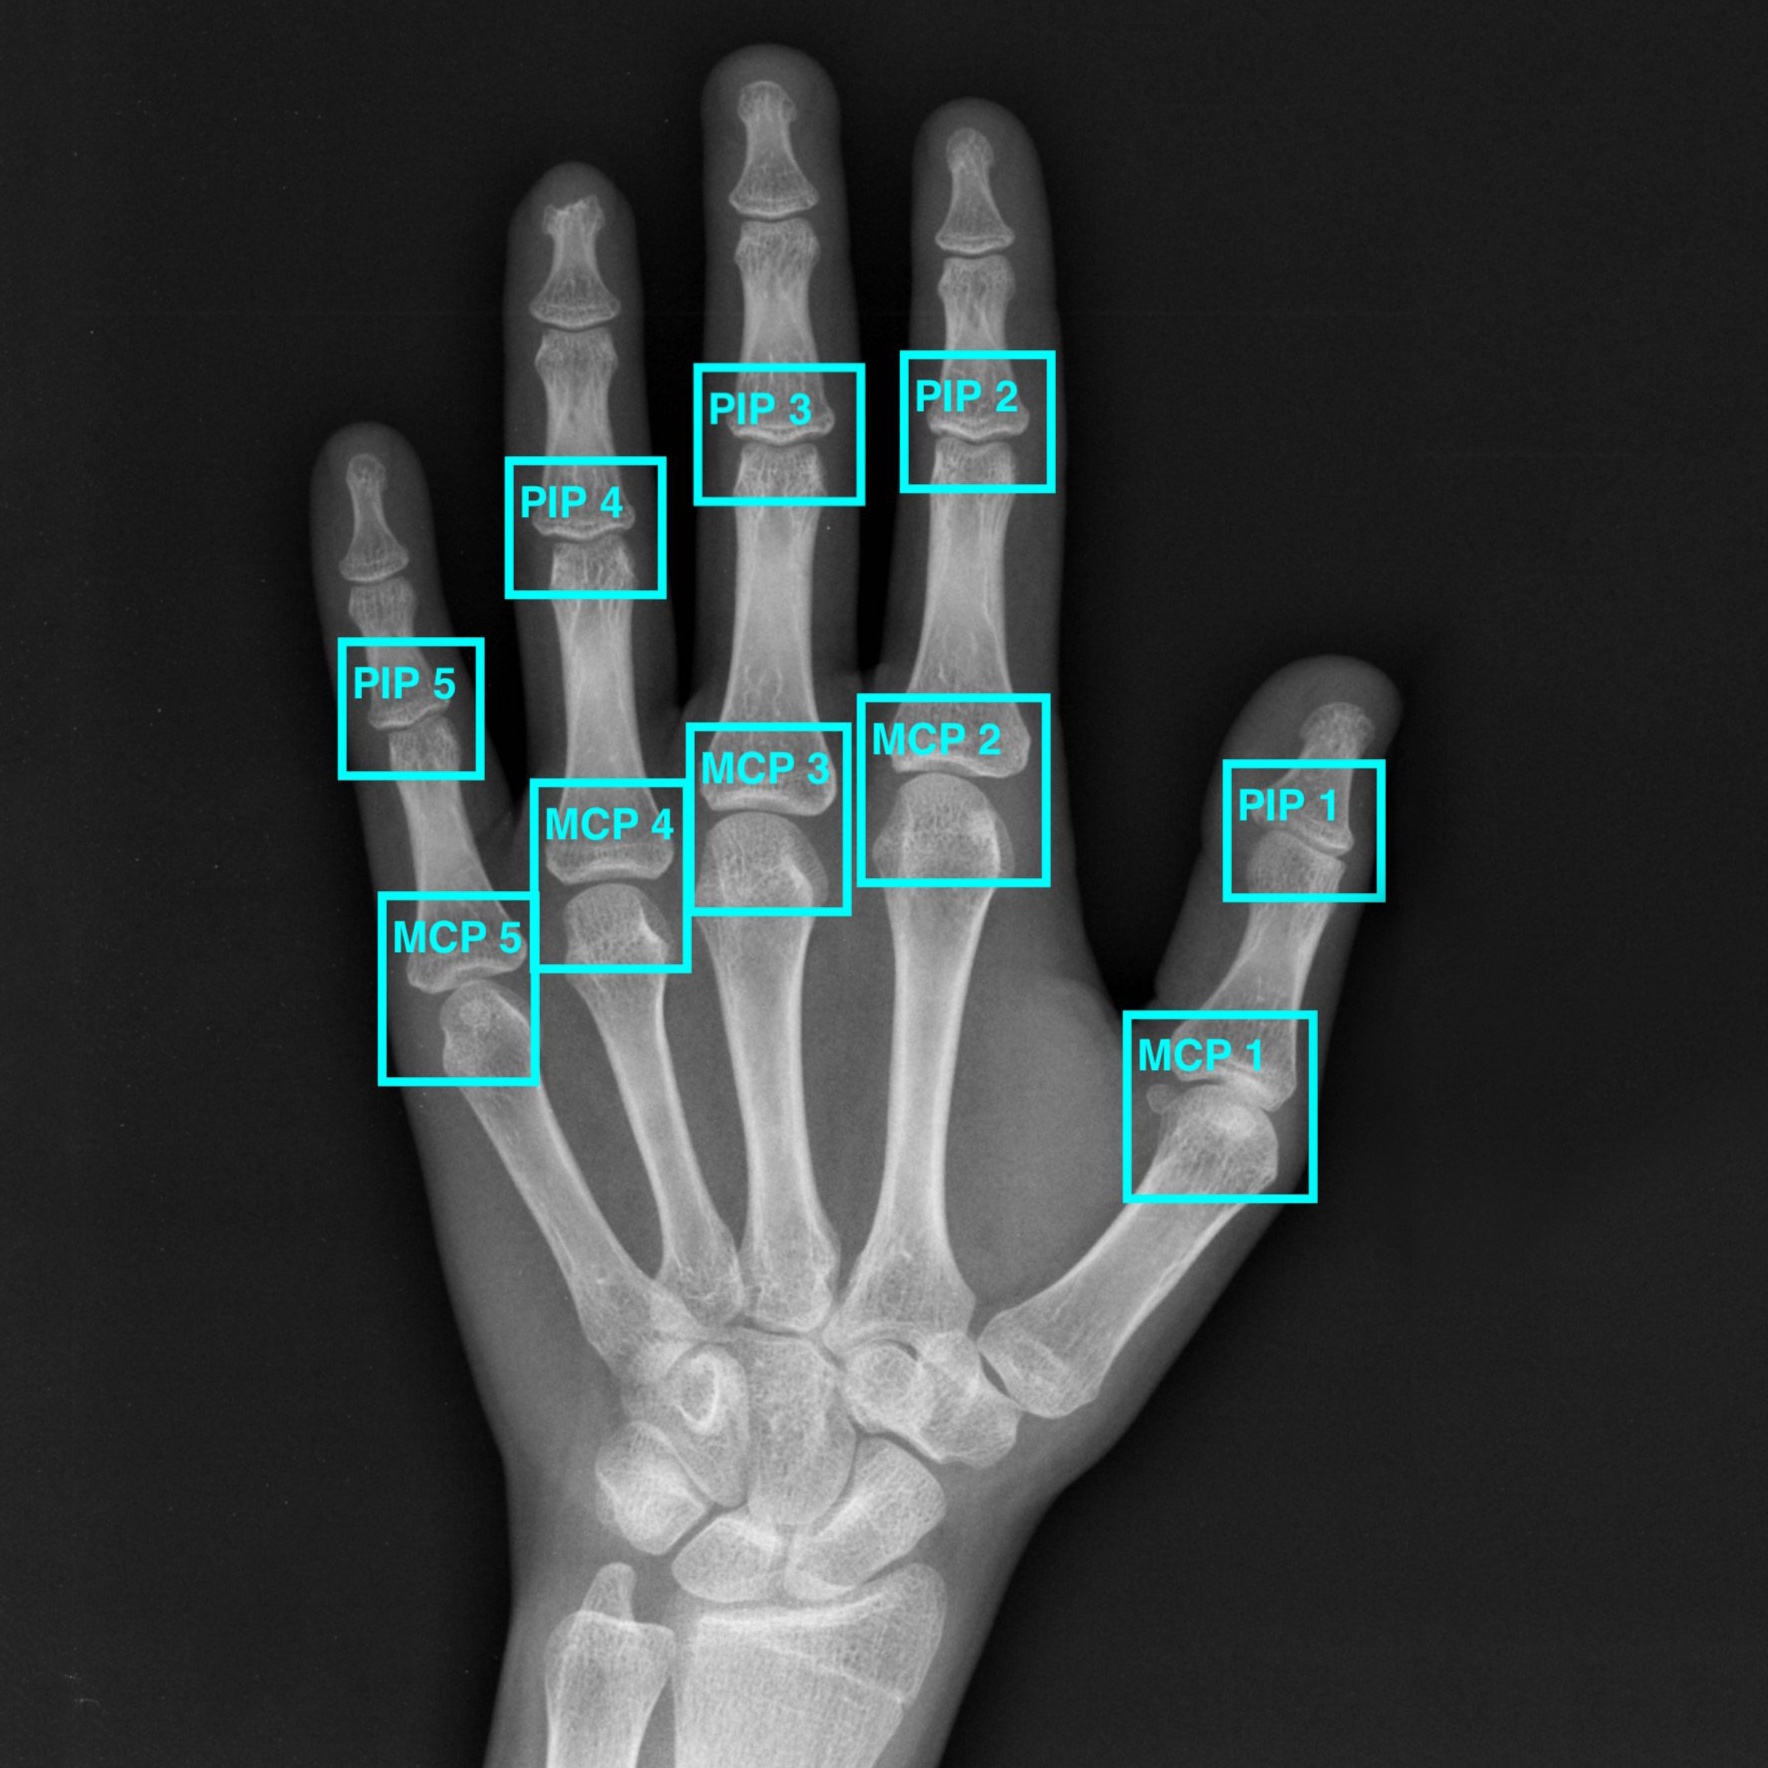
\includegraphics[width=3in]{joints}	
\caption{Proximal interphalangeal (PIP) joints and carpometacarpal  (MCP) joints of the left hand. Cropped images of these ten joints were used to train the neural networks.}
\floatfoot{Original image by Nevit Dilmen (CC BY-SA) \url{https://commons.wikimedia.org/wiki/File:Medical\_X\-Ray\_imaging\_OPC06\_nevit.jpg}}
\label{fig:joints}
\end{figure}

\subsection{Ratingen-score}
\label{subsec:ratingen}

The most important criteria for the effectiveness of a treatment is the influence on the radiological progression. To quantify the irreversible bone erosion in the joint, several scoring methods were developed. The score used in this thesis is called Ratingen-score, it estimates the percentage of eroded joint surface. \cite{rau_2007}. The labels of our data lie within 0 and 100 and correspond to the percentage of joint surface erosion. These values can easily be converted to Ratingen-Scores according to \autoref{tab:ratingen}.


\begin{table}[ht]
\centering
\caption{Disease stages of the Ratingen-score \cite{rau_2007}. The Ratingen-scores are used as labels for the classification model, whereas the percentage of bone erosion is used for the regression model.}
\label{tab:ratingen}
\begin{tabular}{@{}ll@{}}
\toprule
Stage & Description                                                          \\ \midrule
0     & Normal joint                                                         \\
1     & One or more erosions, less than 20 \% of the joint surface is eroded \\
2     & 21 \% - 40 \% of the joint surface is eroded                         \\
3     & 41 \% - 60 \% of the joint surface is eroded                         \\
4     & 61 \% - 80 \% of the joint surface is eroded                         \\
5     & More than 80 \% of the joint surface is eroded                       \\ \bottomrule
\end{tabular}
\end{table}

\subsection{Rau-score}
\label{subsec:rau}

This score is an overall score, which is calculated from the individual Ratingen-scores. The sum of the Ratingen-scores for all 32 joints (5 PIP, 5 MCP and 1 wrist joint per hand and 5 joints per foot) is multiplied by 38 and divided by the number of scored joints.

\subsection{Disease activity score}
\label{subsec:das}

The disease activity score (DAS28) measures the disease activity for the following 28 joints. 5 PIP, 5 MCP and 1 wrist joint per hand plus elbow, shoulder and knee joints \cite{runmc}. The score is derived from the following four measurements.

\begin{enumerate}[label=(\alph*)]
\item $n_s =$ Number of swollen joints
\item $n_t =$ Number of tender joints
\item $ESR$ (erythrocyte sedimentation rate) in mm/hr or \\ $CRP$ (C reactive protein) in mg/L\\ Both measurements are blood markers of inflammation
\item $g_h$ in mm $=$ Patients global assessment of disease activity on a 100 mm long scale from very good (0 mm) to very bad (100 mm).
\end{enumerate}

The DAS28 score is then calculated as follows. \cite{runmc_formula}
\\
\\
$DAS28_{ESR} = 0.56 * \sqrt{n_t} + 0.28 * \sqrt{n_s} + 0.7 * \ln{(ESR)} + 0.014 * g_h$
\\
\\
$DAS28_{CRP} = 0.56 * \sqrt{n_t} + 0.28 * \sqrt{n_s} + 0.36 * \ln{(CRP + 1)} + 0.014 * g_h + 0.96$
\\
\\
\begin{tabular}{@{}lllll}
$DAS28$ & $>$ & $5.2$ & $=$ & high disease activity \\
$DAS28$ & $<$ & $3.2$ & $=$ & low disease activity \\
$DAS28$ & $<$ & $2.6$ & $=$ & remission
\end{tabular}

\subsection{Artificial neural networks}
\label{subsec:ann}
This section offers a very brief introduction to artificial neural networks. A more in-depth explanation can be found in Andrey Karpathy's course notes for the Stanford class CS231n. \cite{karpathy}

The structure of an Artificial neural network (ANN) is inspired by the human brain. A brain consists of approximately 100 billion neurons which form an interconnected network. The neurons can communicate with each other by transmitting electrical potential. If the potential in a neuron reaches a certain threshold, it fires and transmits the potential to connected neurons. \cite{kruse_2016}

An ANN is a very simplified model of this biological process. A single neuron can be described by the following equation. $$f\left(\sum_{i}w_i*x_i+b\right)$$ Where $x_i$ are the inputs, $w_i$ are the weights and $b$ is a bias term. The activation function $f$ models the firing of the neuron.

These single neurons can then be combined to networks. The most simple network is the fully connected neural network described in the following section.

\subsubsection{Fully connected neural networks}
\label{subsubsec:fcnn}
A fully connected neural network (FCNN) has an input layer, arbitrarily many hidden layers and one output layer. The neurons of each layer are connected to every neuron of the next layer. The data  can only flow in one direction, from the input layer towards the output layer. \autoref{fig:fcnn} shows a possible structure for a FCNN.

\begin{figure}[ht]
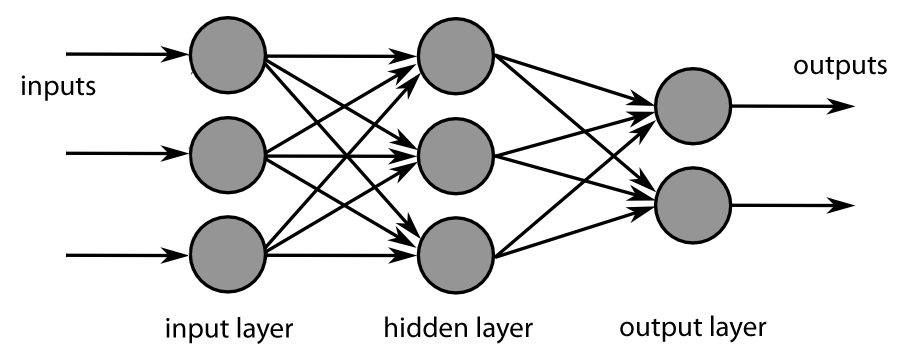
\includegraphics[width=3in]{ffnn}	
\caption{Fully connected neural network with one hidden layer. Networks with many hidden layers are called deep neural networks. The convolutional neural network is a special type of the FCNN.}
\floatfoot{Image by Chrislb (CC BY-SA) \url{https://commons.wikimedia.org/wiki/File:MultiLayerNeuralNetworkBigger_english.png}}
\label{fig:fcnn}
\end{figure}

The number of neurons per layer specifies the width of the neural network, whereas the number of hidden layers specifies the depth of a neural network. A neural network with many hidden layers is called a deep neural network.

For supervised learning the weights and biases of this network can be trained by using back-propagation. The input is fed through the network with randomly initialized parameters. The output is then compared to the true values by using a loss-function. The loss is then back-propagated through the network to adjust the parameters. With every training step, this process is repeated and the loss decreases. This process is also called learning. And for deep neural networks we speak of deep learning.

A special type of the FFNN, used for image recognition, is the convolutional neural network, which is described in the next section.

\subsubsection{Convolutional neural networks}
\label{subsubsec:cnn}
Convolutional neural networks (CNNs) take an image as an input. The image can be seen as a 3-dimensional matrix, where the third dimension includes the different color channels. Instead of fully connected layers, convolutional layers are used. Convolutions work as filters that detect different features in the image. These filters usually have a small size (e.g. 3x3) and are moved over the image. \autoref{fig:cnn} shows a possible architecture of a CNN with multiple convolutional layers and a fully connected layer at the end.

\begin{figure}[ht]
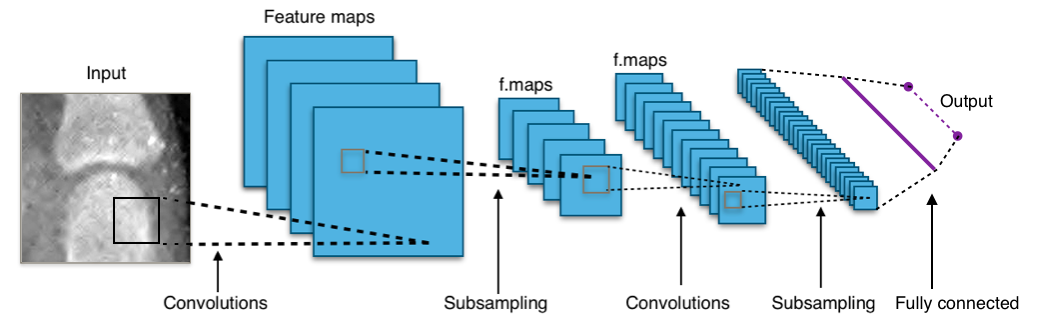
\includegraphics[width=5in]{cnn}	
\caption{Example structure of a convolutional neural network. Convolutions are filters that are moved over the image and automatically extract features. The fully connected layers at the end use those features to do classification or regression.}
\floatfoot{Original  image by Aphex34 (CC BY-SA) \url{https://commons.wikimedia.org/wiki/File:Typical_cnn.png}}
\label{fig:cnn}
\end{figure}


In contrast to classical machine learning we there is no need to extract features beforehand. The hidden layers of the deep convolutional neural network will do the feature extraction automatically.

The deep convolutional neural networks used in this thesis are built from the following layers:

\begin{enumerate}[label=(\alph*)]
\item \textbf{Input layer} First layer of the network with the dimensions of the input image. E.g.  150 x 150 x 1 for greyscale images with only one color channel or 150 x 150 x 3 for RGB images with three color channels.
\item \textbf{Convolutional layer} These layers consist of multiple filters that are moved over the image and automatically extract features from the previous layer.
\item \textbf{Batch normalization layer} This layer adds a batch-wise normalization to the network that helps it to converge faster. It also regularizes the network similar to a dropout layer. A detailed description of batch normalization can be found in the article by Ioffe and Szegedy \cite{ioffe_2015}.
\item \textbf{Activation layer} For the hidden layers, the ReLu activation function was used, it is calculated as follows: $f(x) = max(0, x)$\\ For the output layer in the classification model the softmax activation function was used, it is calculates as follows: $f_i(z) = \frac{e^{z_i}}{\sum^{N}_{k=1} (e^{z_k})}, \text{	    for    } i = 1, 2, .., N$ \cite{softmax} This function transforms the values of the output vector into the the range [0, 1]. In addition all values of the vector add up to one. \\ For the output layer in the regression model the sigmoid activation function is used. It is calcualted as follows: $f(x) = \frac{1}{1 + e^{-x}}$ \cite{sigmoid} This function transforms all values of the output vector into the range [0, 1].
\item \textbf{Max pooling layer} This layer is used for dimensionality reduction. Max pooling downsamples areas of e.g. 2 x 2 into 1 x 1, only the maximum of the four input values is kept. This reduces the width and height of the previous layer.
\item \textbf{Dropout layer} This layer adds regularization to the fully connected layers, which helps to prevent overfitting. In the training phase, e.g. 50 \% of the neurons are randomly disabled.
\item \textbf{Fully connected layer} One or more of these layers are added at the end of the CNN to compute the class or regression scores.
\item \textbf{Output layer} The last layer of the network is a fully connected layer with as many neurons as labels. (e.g. 6 neurons for the 6 Ratingen-scores)
\end{enumerate}


\newpage
\section{Data}
\label{sec:data}

The received data consists of jpg images of the joints and two csv datasets. The main dataset includes the following relevant columns shown in \autoref{tab:main_dataset}.

\begin{table}[ht]
\centering
\caption{Description of the relevant columns of the main dataset}
\label{tab:main_dataset}
\begin{tabular}{@{}ll@{}}
\toprule
Column name   & Description                                           \\ \midrule
id\_x         & Unique observation id                                 \\
patient\_id   & Unique patient id                                     \\
date\_x       & Date of the consultation                              \\
date\_y       & Date on which the joints were scored                  \\
sop\_iuid     & Unique x-ray image id                                 \\
body\_part    & Left/right hand/foot or both hands/feet               \\
hand\_left\_x & Percentage of bone erosion for joint x                \\
rau\_score    & Overall Rau-score described in \autoref{subsec:rau} \\ \bottomrule
\end{tabular}
\end{table}

This is the dataset where the percentages of bone erosion for the joints of the left hand were extracted. The corresponding x-ray image can be found by using the sop\_iuid.

The secondary dataset contains additional scores which only exist for some of the patients and some consultations. A description of the relevant columns is shown in \autoref{tab:sec_dataset}. The two datasets can be merged on patient\_id and date/date\_x.

\begin{table}[ht]
\centering
\caption{Description of the relevant columns of the secondary dataset. The two datasets can be merged on patient\_id and date/date\_x.}
\label{tab:sec_dataset}
\begin{tabular}{@{}ll@{}}
\toprule
Column name   & Description                                           \\ \midrule
patient\_id   & Unique patient id                                     \\
date       & Date of the consultation                              \\
physician\_global & Medical global assessment of disease activity\\
\_disease\_activity    \\   
global\_patient & Patient estimate of disease activity   \\
\_estimate\_disease\_activity    \\ 
das28bsr\_score    & DAS28BSR as described in \autoref{subsec:das}             \\
das283crp\_score & DAS28ERP as described in \autoref{subsec:das} \\ \bottomrule
\end{tabular}
\end{table}


The images of the joints were already extracted from all the x-ray images of left hands. In total there were 102'265 images of single joins available.


\subsection{Data preparation}
\label{subsec:data_prep}

The data preparation step brings the jpg images into a suitable format that can be used as an input for the CNN. 

The original images have values between 0 and 255. We divided the data by 255 in order to have inputs in the range of [0,1].

The data was randomly split into a training set (70 \% of the data), a validation set (20 \% of the data) and a test set (10 \% of the data). It was split such that all images of the same patient are in the same set.

The images of the joints have varying exposure. Some images are very dark while others are very bright. It was therefore considered to apply a histogram equalization, which is a linear transformation that maps the lightest pixel to 1 and the darkest pixel to 0. However, this transformation did not improve the accuracy of the models and was not used for the final models.

The bone erosion scores of the labeled joints are highly imbalanced. As seen in \autoref{fig:imbalance} most of the joints are healthy and received a score of 0. There are also a lot of observations with little bone erosion with scores between 0 and 25. There are very little observations with scores higher than 25. Only the fully eroded joints with a score of 100 seem to be a bit more frequent.

\begin{figure}[ht]
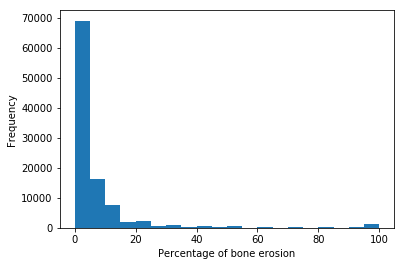
\includegraphics[width=3in]{imbalance}	
\caption{Histogram of the bone erosion scores for the 102'265 images of joints. The scores are highly imbalanced with most observations being healthy joints with score 0. To compensate for the imbalance a weighted loss function and oversampling of the underrepresented classes were considered.}
\label{fig:imbalance}
\end{figure}

When training the CNN, it minimizes the overall loss-function. For imbalanced data the CNN performs bad for the underrepresented part of the data. In this case, the model would be a bad predictor for high scores. In order to make the model a good predictor for all cases, we tried weighting the loss function as well as oversampling the underrepresented classes.

\newpage
\section{Methods and results}
\label{sec:methods&results}

In order to predict the bone erosion scores, different models were considered. This section describes the different steps of the model selection process and the results of the different models. At the end, a final classification model which predicts the Ratingen-score and a final regression model which predicts the percentage of bone erosion were selected.

\subsection{Software and infrastructure}
The models were built in Python 3.5 \cite{python} with the package Tensorflow 1.4 \cite{tensorflow} using the high level API Keras \cite{keras}. For general machine learning the package Scikit-learn \cite{scikit-learn} was used. The package Matplotlib \cite{matplotlib} was used to produce figures. In addition, the programming language R \cite{r} was used for further analysis of the results and for producing figures as well.

For the training of the models a Nvidia Titan X (Pascal) graphics card was used.

\subsection{Base models}

We decided to create a classification as well as a regression model. The architecture of both models is similar, each model has 6 blocks of two convolutional layers of the size 3x3 followed by a max pooling layer. The number of filters per convolutional layer is increasing with every second block, whereas the size of the layers is decreasing due to the max pooling layers. Every convolutional layer uses batch normalization before the ReLu activation function.

This first part is identical for both models. We then flatten the output of the last convolution block and use two dense layers with batch normalization, ReLu activation and dropout. Only the number of neurons in the dense layers is different between the two models. The output layer however is different between the two models and described in the next two sections.

\subsubsection{Classification model}
\label{subsubsec:clas}

The classification model directly predicts the Ratingen-score. The output layer has 6 neurons according to the 6 Ratingen classes (0 - 5). The Softmax activation function is then used to predict the probabilities for each class. The architecture of this CNN is shown in \autoref{fig:cnn_cla}.

\begin{figure}[ht]
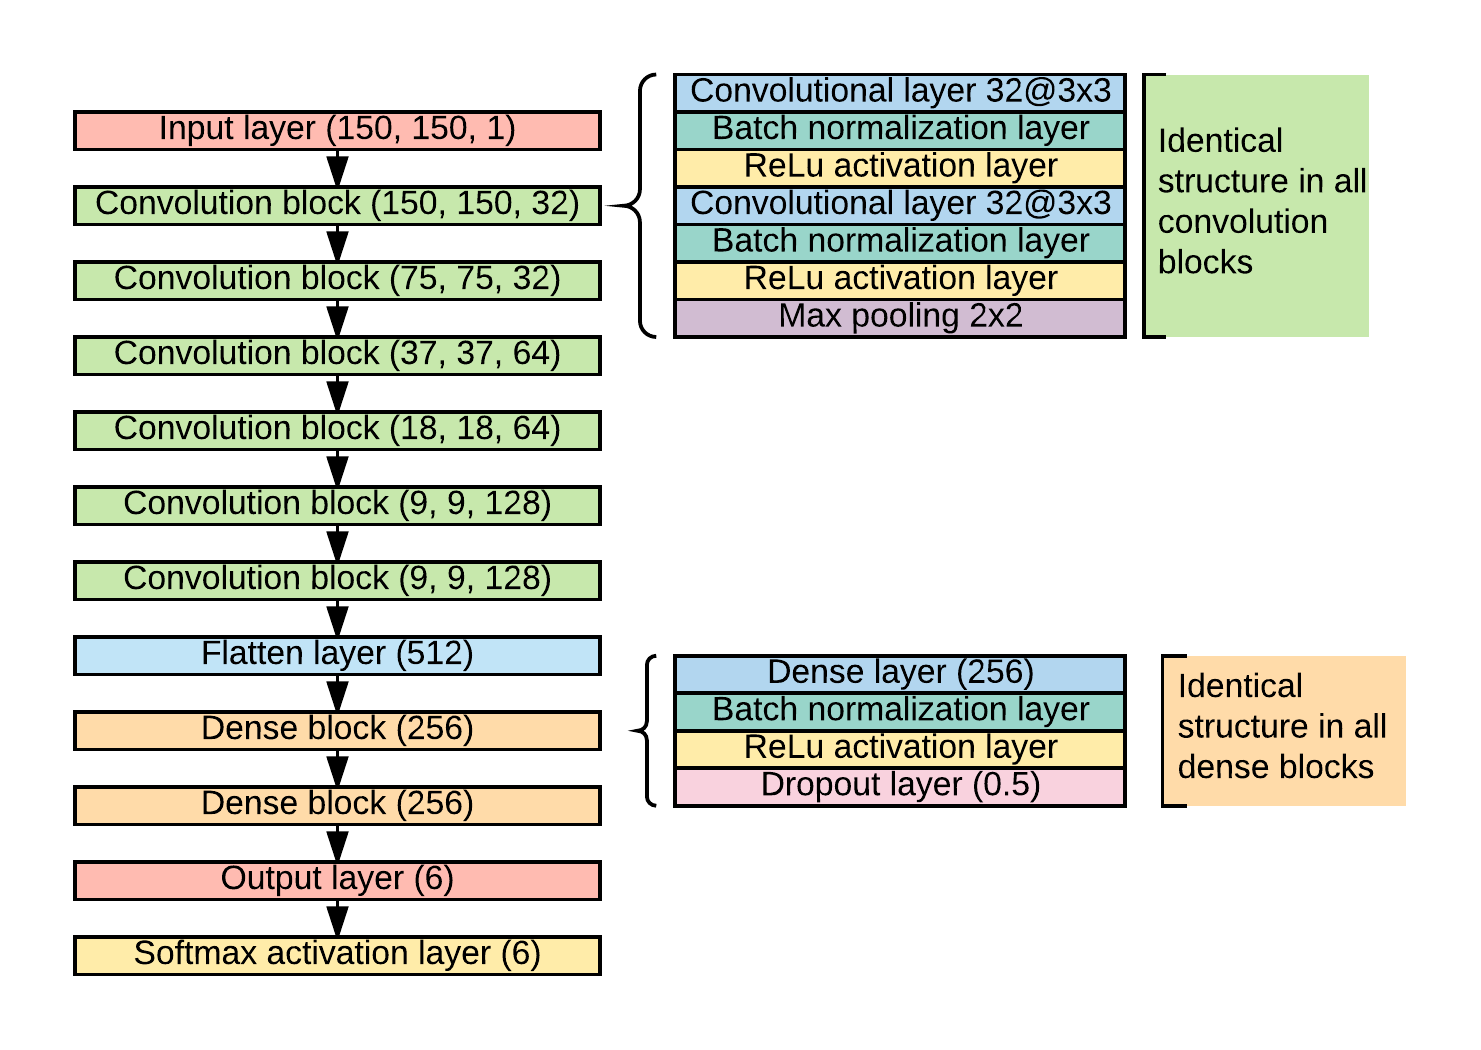
\includegraphics[width=4in]{cnn_classification}	
\caption{Architecture of the CNN for classification. The number of filters is increasing with every other convolutional block, whereas the dimensions of the layers are decreasing with every block due to the max pooling layers.}
\label{fig:cnn_cla}
\end{figure}

The model is trained for 25 epochs with the ADAM optimizer and a learning rate of 0.001. Categorical cross entropy is used as the loss function. The images are fed through the model in batches of 100 images at a time.

As described in \autoref{subsec:data_prep} we tried different approaches to handle the imbalanced data. 

\begin{enumerate}[label=(\alph*)]
\item The first model is trained on the original data and is used as a basis to compare the results of the other models.
\item For the second model we oversampled the underrepresented classes in order to have roughly the same number of images per class. The oversampled images are augmentations of the original data. Random rotations of up to 25 degrees, shearing of up to 0.1 radians and and zooming of up to 10 \% were used.
\item The third model used the same data as the first model, but the loss function was weighted with class weights. The class weights where chosen such that the class weight multiplied by the number of observation in that class equals to the same value for all classes.
\end{enumerate}

Model b) was trained for 25 epochs, whereas the other two models started overfitting and had to be stopped early after 9 epochs. The training and validation loss and accuracy for the three models are shown in \autoref{fig:loss_acc_clas}. The normalized confusion matrices for the validation dataset for the three models can be seen in \autoref{fig:confusion}.

\begin{figure}[ht]
\begin{tabular}{ccc}
\subfloat[Loss]{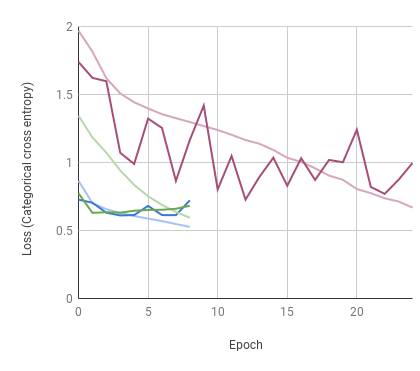
\includegraphics[width = 2.1in]{classification_loss}} &
\subfloat[Accuracy]{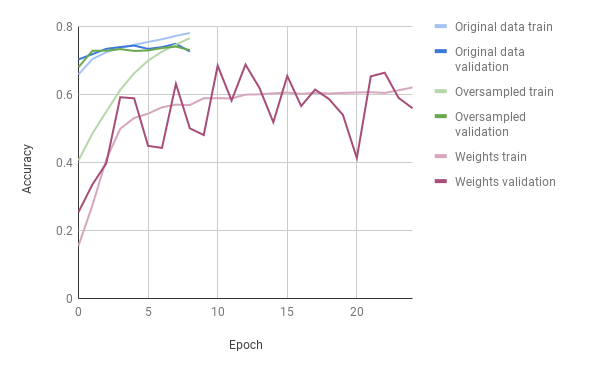
\includegraphics[width = 3in]{classification_accuracy}} &
\end{tabular}
\caption{Training and validation loss and accuracy for the three classification models. The models on original and oversampled data started overfitting and were stopped early after 9 epochs.}
\label{fig:loss_acc_clas}
\end{figure}

\begin{figure}[ht]
\begin{tabular}{ccc}
\subfloat[Original data]{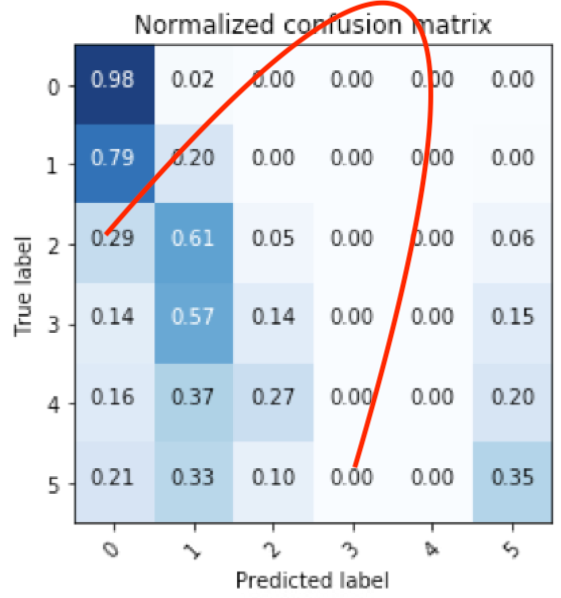
\includegraphics[width = 1.5in]{classification_original}} &
\subfloat[Oversampled]{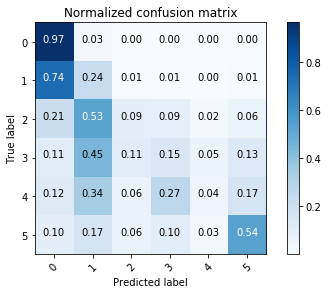
\includegraphics[width = 1.5in]{classification_oversampled}} &
\subfloat[Weights]{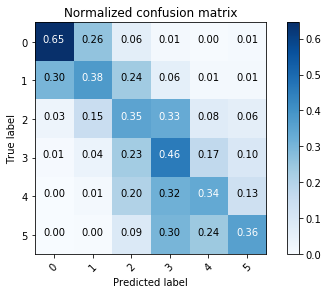
\includegraphics[width = 1.5in]{classification_weights}}
\end{tabular}
\caption{Normalized confusion matrices for the predictions of the classification models on the validation set. Models a) and b) have a higher accuracy but are biased towards the overrepresented classes, whereas the predictions of model c) are better balanced across all labels.}
\label{fig:confusion}
\end{figure}

The evaluation metrics for the three models can be seen in \autoref{tab:metrics_cla}. We discovered that the accuracy is not a suitable metric. Model a) has the highest accuracy but makes a lot of misclassifications in the under-represented classes. Whereas the accuracy of model c) is the lowest, but the accuracy for the underrepresented classes is much better.

Therefore, we decided to use the normalized accuracy as our evaluation metric. It is the mean of the six class accuracies. It describes much better, whether our model is a good predictor for all classes.

As a second metric, we calculated the normalized accuracy for predictions that are in the right class or one class above or below the correct class. This metric takes into account, that a misclassification by 1 is far less severe than a misclassification by 5.

\begin{table}[ht]
\centering
\caption{Evaluation metrics for the classification models. Even though model c) has the worst accuracy, it was selected, because the normalized accuracies are superior to the other models. The normalized accuracy is the mean of the six class accuracies. Normalized $\pm$ 1 accuracy is the normalized accuracy of predictions that are in the right class or one class above or below the correct class.}
\label{tab:metrics_cla}
\begin{tabular}{@{}llll@{}}
\toprule
                                & a)    & b)    & c)    \\ \midrule
Accuracy                        & 0.726 & 0.73 & 0.569 \\
Normalized accuracy       & 0.264 & 0.337 & 0.422 \\
Normalized $\pm$ 1 accuracy  & 0.558 & 0.675 & 0.817 \\ \bottomrule
\end{tabular}
\end{table}

Considering the class normalized accuracies, model c) is clearly superior to the other two models. Therefore, this model was selected as the base model for the classification task.

\subsubsection{Regression model}
\label{subsubsec:reg}


For the regression model, we decided to predict the discrete cumulative density function (CDF) instead of predicting directly the bone erosion score. The model is only slightly different from the classification model. The output layer has 101 neurons for the discrete integer bone erosion scores from 0 to 100. Since the output layer has much more neurons compared to the classification model, the number of neurons in the dense layers were also increased. Since the outputs still have to lie within [0, 1] but do not have to sum up to 1, the sigmoid activation function is used instead of the softmax activation function.This architecture can be seen in \autoref{fig:cnn_reg}.

\begin{figure}[ht]
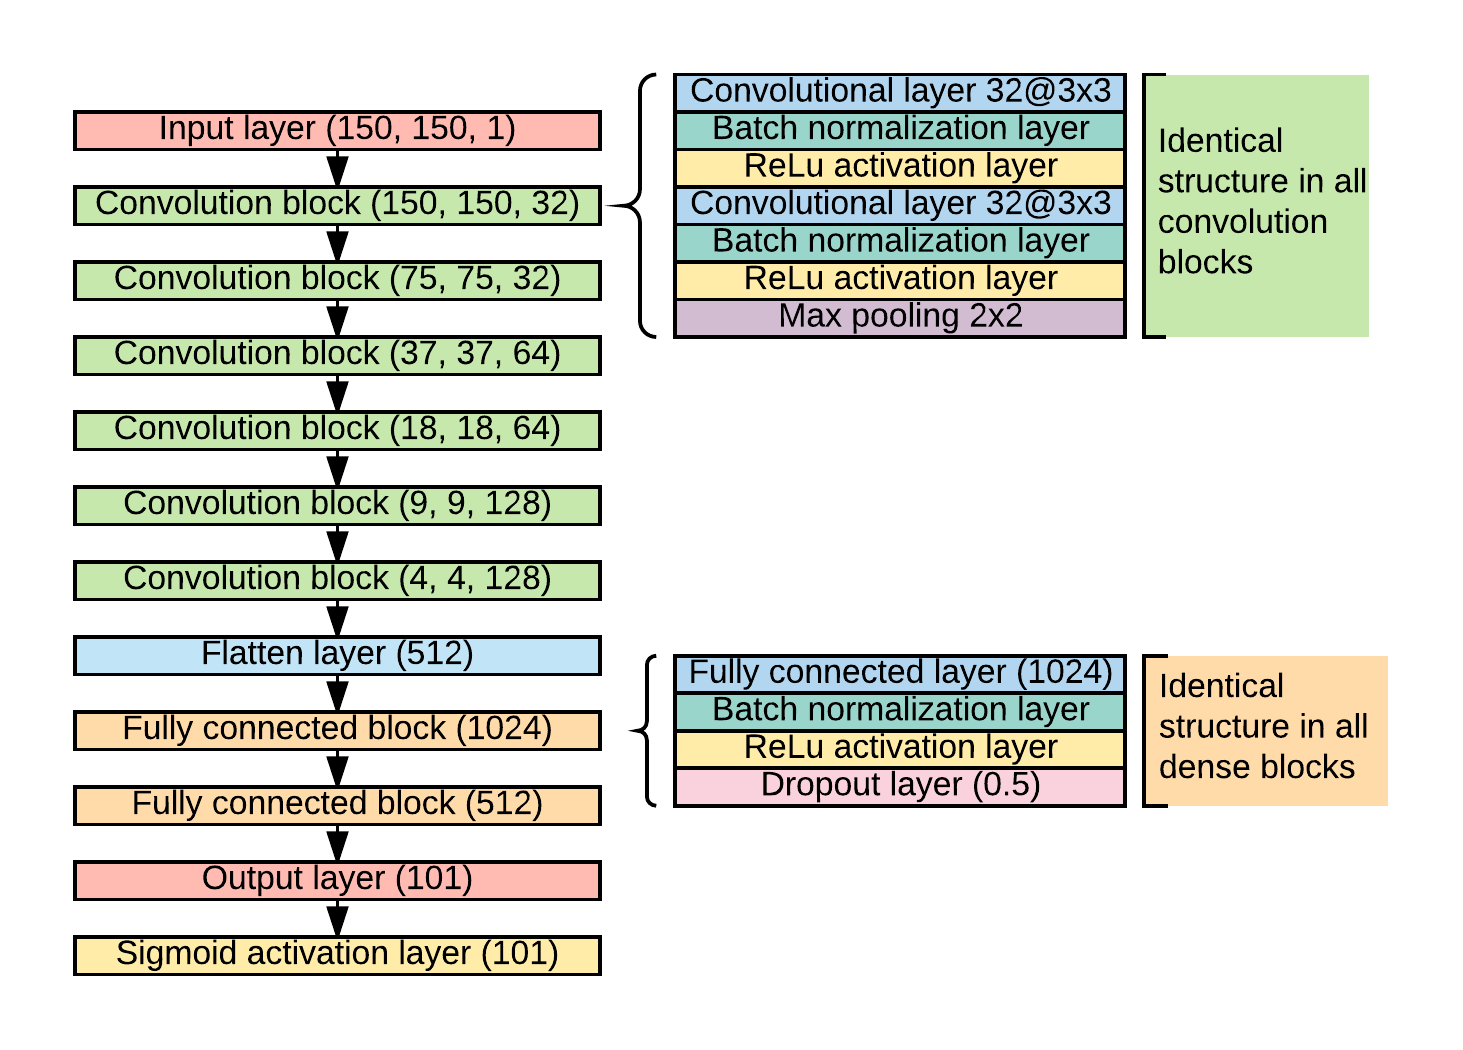
\includegraphics[width=4in]{cnn_regression}	
\caption{Architecture of the CNN for regression. The only differences to the classification model are the number of neurons in the dense and output layers and the activation function of the output layer.}
\label{fig:cnn_reg}
\end{figure}

To train the model, the Continuous Ranked Probability Score (CRPS) was used as the loss function. For the discrete case it is calculated as follows. \cite{crps}

$$CRPS = \frac{1}{101 * N} \sum\limits_{n=1}^{N} \sum\limits_{k=0}^{101} (P(y \geq k) - H(k - R_n))^2$$

Where $P$ is the predicted distribution, $N$ is the number of observations, $R$ is the actual percentage of bone erosion and $H(x) = \begin{cases}
1 & \text{for $x \geq 0$,}\\
0 & \text{otherwise.}
\end{cases}$ \cite{crps}

The blue area visualized in \autoref{fig:crps} shows the error between the predicted distribution and the actual percentage of bone erosion. This error is measured with the CRPS. \cite{crps}

\begin{figure}[ht]
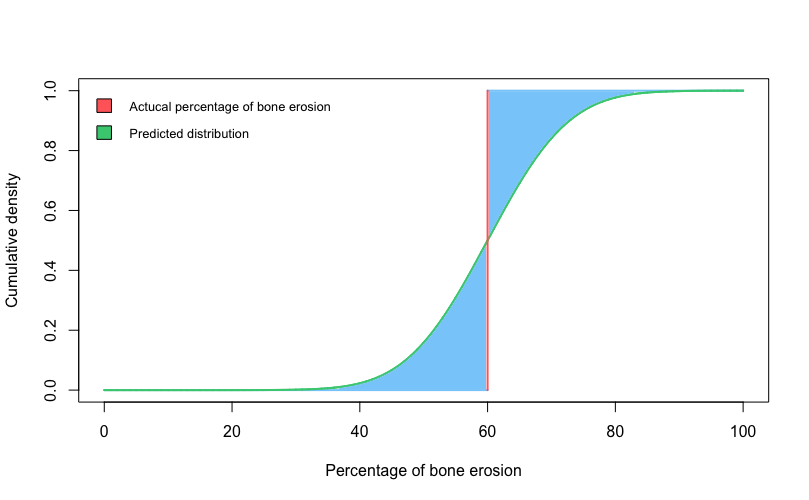
\includegraphics[width=10cm]{crps}	
\caption{The blue area shows the error between the predicted distribution and the actual percentage of bone erosion. This error is measured with the CRPS.}
\label{fig:crps}
\end{figure}

The model predicts the discrete CDF for the percentage of bone erosion. An example of a prediction is shown by the blue dots in \autoref{fig:crps_pred}. The green line shows the true label whereas the red line shows the expected value of the predicted distribution. The expected value of our discrete CDF is calculated as follows. $E(x) = \sum_{i=1}^{101} \left ( 1 - p_i \right )$, where $p_i$ are the 101 predictions.

\begin{figure}[ht]
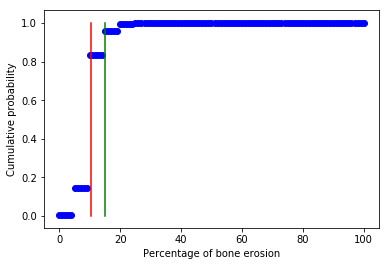
\includegraphics[width=3in]{crps_pred}	
\caption{Example of a prediction. The blue dots show the 101 predictions for the CDF. The red line is the expected value of that CDF and the green line is the true label.}
\label{fig:crps_pred}
\end{figure}

This model was trained on the original data, oversampled data and with a weighted loss function in the same way as described in \autoref{subsubsec:clas}. This time all three models were trained for 25 epochs, as they did not start overfitting. The train and validation loss and mean absolute error (MAE) can be seen in \autoref{fig:loss_acc_reg}. The MAE is calculated for the predictions of the CDF and not for the final labels. \autoref{fig:hexbin} shows 2D histograms of the predictions for the validation set for the three models. 

\begin{figure}[ht!]
\begin{tabular}{ccc}
\subfloat[Loss]{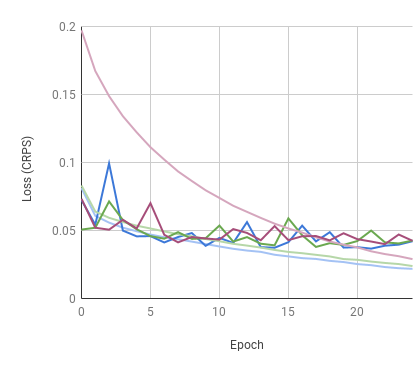
\includegraphics[width = 2.1in]{regression_loss}} &
\subfloat[Accuracy]{\includegraphics[width = 3in]{regression_MAE}}
\end{tabular}
\caption{Training and validation loss and mean absolute error for the three regression models. The three models were trained for 25 epochs. The MAE is calculated for the predictions of the CDF.}
\label{fig:loss_acc_reg}
\end{figure}


\begin{figure}[ht!]
\begin{tabular}{cc}
\subfloat[Original data]{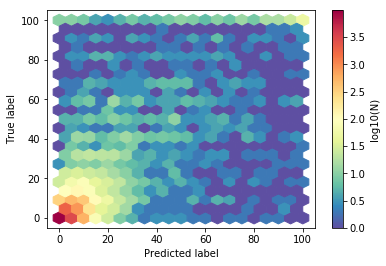
\includegraphics[width = 2.5in]{regression_original}} &
\subfloat[Oversampled]{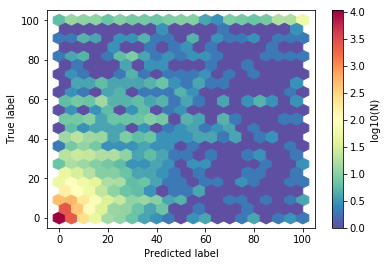
\includegraphics[width = 2.5in]{regression_oversampled}} \\
\subfloat[Weights]{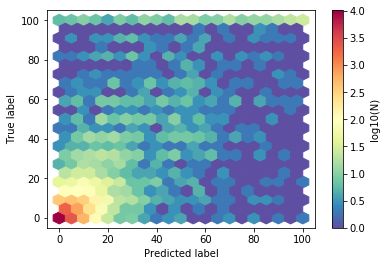
\includegraphics[width = 2.5in]{regression_weights}}
\end{tabular}
\caption{2D histograms of the predictions of the regression models on the validation set. The colors are on a logarithmic scale with base 10. All models are bad predictors for the joints with a true label of 100.}
\label{fig:hexbin}
\end{figure}

There is no big visual difference between the three plots. All three models are predicting badly for the joints with true labels of 100.

In contrast to \autoref{fig:loss_acc_reg}, where MAE is calculated for the predictions of the CDF, the MSE and MAE in the evaluation metrics in \autoref{tab:metrics_reg} are calculated for the final predictions. We can see, that model a) has the smallest CRPS, smallest mean squared error (MSE) as well as the smallest mean absolute error (MAE) of the three models. Therefore we decided to use model a) as the base model for regression.

\begin{table}[ht]
\centering
\caption{Evaluation metrics for regression. The MSE and MAE are calculated for the bone erosion scores, whereas the CRPS is calculated for the predicted distributions. Model a) was selected since it has the best CRPS, MSE and MAE.}
\label{tab:metrics_reg}
\begin{tabular}{@{}llll@{}}
\toprule
                                & a)    & b)    & c)    \\ \midrule
CRPS							& 0.0291 & 0.0304 & 0.0426 \\
Mean squared error (MSE)        & 80.884 & 83.017 & 94.488 \\
Mean absolute error (MAE)       & 4.046 & 4.072 & 4.057 \\

\bottomrule
\end{tabular}
\end{table}

\FloatBarrier

\subsection{Transfer learning}
\label{subsec:transfer_learning}

Tajbakhsh et al. \cite{tajbakhsh_2017} stated in their paper that pre-trained networks with fine-tuning always outperformed or at least performed as well as CNNs trained from scratch. We examined whether transfer learning could improve our predictions by using the Inception V3 model \cite{szegedy_2015} which was pre-trained on the Imagenet dataset. We used the pre-trained weights and cut off the output layer. Instead we added two dense layers and an output layer identical to the output layers described in \autoref{subsubsec:clas} and \autoref{subsubsec:reg} for the classification and regression models respectively. \autoref{fig:transfer_learning} shows the architecture of the two models. Since the model was trained on color images, the greyscale images were converted to RGB. The Inception V3 model further requires the input data to be transformed to [-1,1] which was done in an additional pre-processing step.

\begin{figure}[ht]
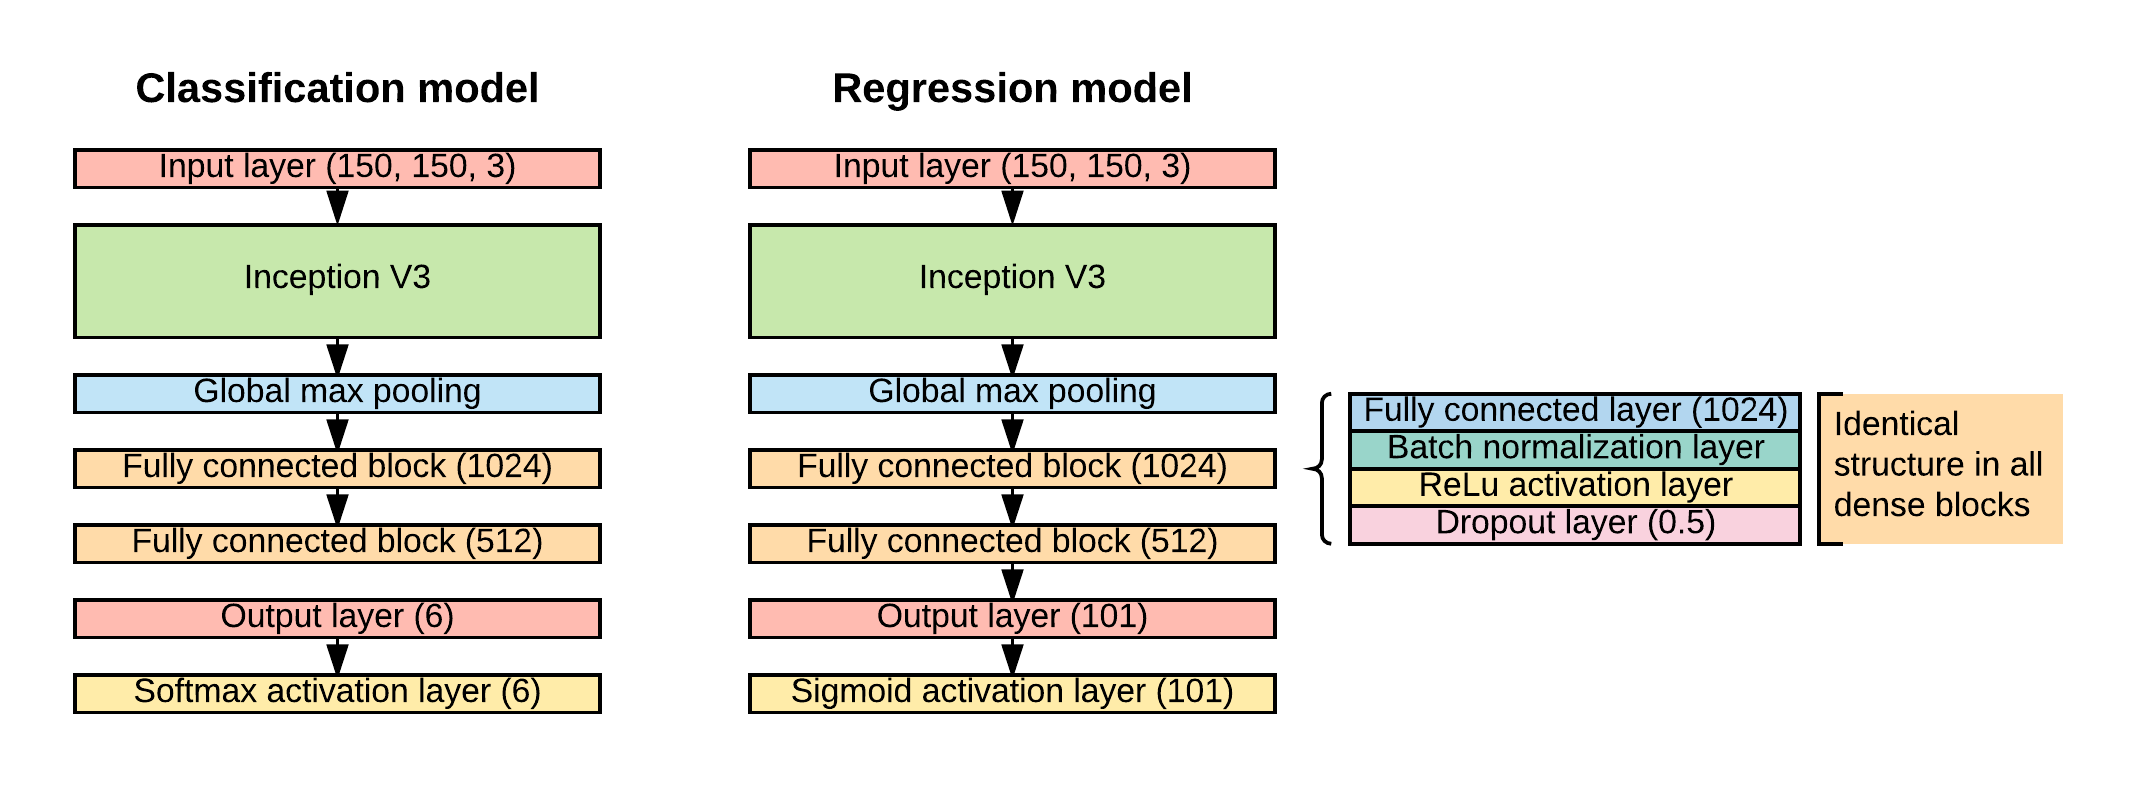
\includegraphics[width=4in]{transfer_learning}	
\caption{Model architecture for transfer learning. The Inception V3 model is used with pre-trained weights on the Imagenet dataset. The input layer now has 3 color channels since the model was trained on RGB images. The dense layers are similar to the previous models but with more neurons. The output layers are identical to the existing models.}
\label{fig:transfer_learning}
\end{figure}

For the training, all existing weights were frozen and only the dense layers and the output layer were trained for 25 epochs. Again, the ADAM optimizer was used but with a learning rate of 0.0001, which is ten times smaller than the learning rate used in the previous models. Afterwards we repeated the training for all layers for an additional 25 epochs. The train and validation loss and accuracy/MAE are shown in \Cref{fig:loss_acc_transfer_cla,fig:loss_acc_transfer_reg}. 

\begin{figure}[ht!]
\begin{tabular}{ccc}
\subfloat[Loss]{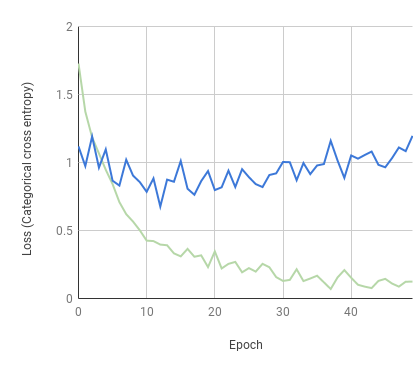
\includegraphics[width = 2.1in]{transfer_cla_loss}} &
\subfloat[Accuracy]{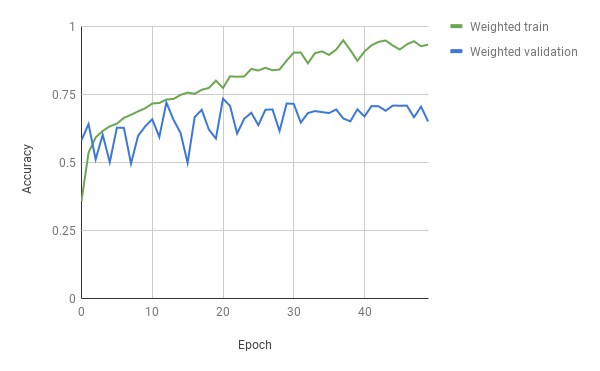
\includegraphics[width = 3in]{transfer_cla_acc}}
\end{tabular}
\caption{Training and validation loss and accuracy for the transfer learning classification model. The first 25 epochs show the training of the dense layers whereas the second half of the training includes all layers.}
\label{fig:loss_acc_transfer_cla}
\end{figure}

It seems that the transfer learning model for classification did not learn much after the first few epochs. The loss stays almost equal during the whole training and even increases a bit towards the end. The accuracy increases only slightly.

\begin{figure}[ht!]
\begin{tabular}{ccc}
\subfloat[Loss]{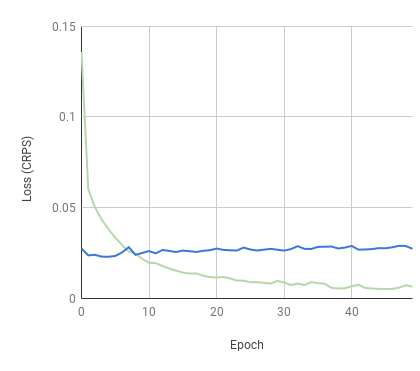
\includegraphics[width = 2.1in]{transfer_reg_loss}} &
\subfloat[Accuracy]{\includegraphics[width = 3in]{transfer_reg_MAE}}
\end{tabular}
\caption{Training and validation loss and accuracy for the transfer learning regression model. The first 25 epochs show the training of the dense layers whereas the second half of the training includes all layers.}
\label{fig:loss_acc_transfer_reg}
\end{figure}

The transfer learning model for regression behaved similarly. The loss stays more or less equal during the whole training and the mean absolute error decreases only slightly after the first few epochs.

The predictions for the validation set are shown in \autoref{fig:transfer_learning_results}. When comparing the normalized confusion matrix of the transfer learning classification model with model c) in \autoref{fig:confusion}, we can see that the transfer learning model has the higher accuracy for the extreme cases 0, 1 and 5. However, the model seems to perform worse for the Ratingen-scores 2, 3 and 4. 

The 2D histogram of the transfer learning regression model can be compared to a) in \autoref{fig:hexbin}. It is apparent that the transfer learning model is better at predicting the very bad cases with scores of 100. There are still a few outliers, but far fewer than in the base regression model.

\begin{figure}[ht]
\begin{tabular}{cc}
\subfloat[Classification]{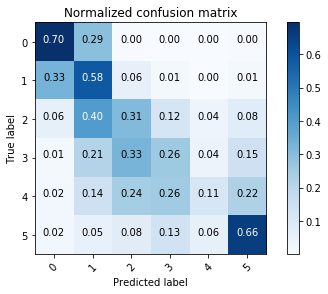
\includegraphics[width = 2.5in]{transfer_learning_classification}} &
\subfloat[Regression]{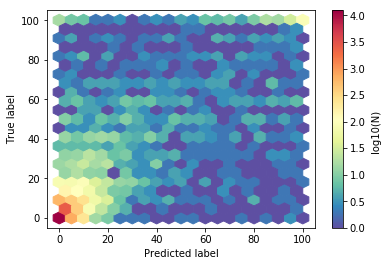
\includegraphics[width = 2.5in]{transfer_learning_regression}}
\end{tabular}
\caption{Normalized confusion matrix for the predictions of the transfer learning classification model on the validation set. And a 2D histogram for the predictions of the transfer learning regression model with colors on a logarithmic scale with base 10.}
\label{fig:transfer_learning_results}
\end{figure}

\autoref{tab:transfer_learning_metrics} shows the evaluation metrics for the two transfer learning models. To compare the metrics of the transfer learning classification model with the base classification model, Wilson score intervals on the 5 \% significance level were computed. The Wilson score intervals for the normalized accuracy of the base model and the transfer learning model are (0.415, 0.429) and (0.43, 0.443) respectively. This means that the transfer learning model is slightly better. The Wilson score intervals for the second metric, the normalized $\pm$ 1 accuracy are (0.812, 0.823) for the base model and (0.781, 0.793) for the transfer learning model. Here the base model is better. Since the transfer learning model for classification only brings a very small improvement in the normalized accuracy and worsens the normalized $\pm$ 1 accuracy, we decided to keep the base classification model over the transfer learning model.

The metrics of the transfer learning regression model can be compared with a) in \autoref{tab:metrics_reg}. The transfer learning model is considerably better than the base regression model. The CPRS decreases from 0.029 to 0.027, the MSE improves from 80.9 to 72.8 and the MAE from 4.0 to 0.7. Therefore we decided to keep the new transfer learning model over the base regression model.

\begin{table}[ht!]
\begin{tabular}{cc}
\begin{tabular}{@{}ll@{}}
\toprule
                                & Classification \\ \midrule
Accuracy                        & 0.65           \\
Normalized accuracy       & 0.436          \\
Normalized $\pm$ 1 accuracy  & 0.787          \\ \bottomrule
\end{tabular}
\quad
\begin{tabular}{@{}ll@{}}
\toprule
        & Regression \\ \midrule
CRPS    & 0.0274          \\
MSE     & 72.768          \\
MAE		& 3.119          \\ \bottomrule
\end{tabular}
\end{tabular}
\caption{Evaluation metrics for the transfer learning models. The normalized accuracy is the mean of the six class accuracies. Normalized $\pm$ 1 accuracy is the normalized accuracy of predictions that are in the right class or one class above or below the correct class. The MSE and MAE are calculated for the bone erosion scores, whereas the CRPS is calculated for the predicted distributions.}
\label{tab:transfer_learning_metrics}
\end{table}

\subsection{Model evaluation}
\label{subsec:evaluation}

We have now found the best models for classification and regression. Those two final models are now evaluated on the test set. The normalized confusion matrix for the predictions of the base classification model and the 2D histogram for the predictions of the transfer learning model for the test set are shown in \autoref{fig:eval}.

\begin{figure}[ht!]
\begin{tabular}{cc}
\subfloat[Classification]{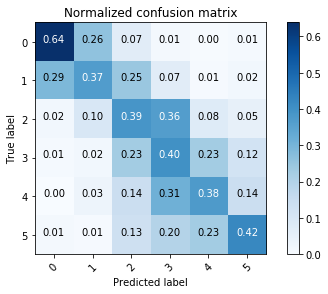
\includegraphics[width = 2.5in]{clas_val}} &
\subfloat[Regression]{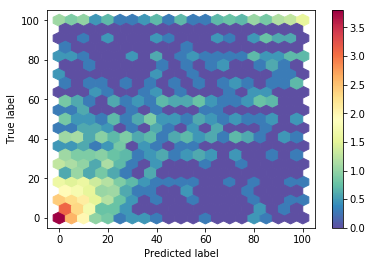
\includegraphics[width = 2.5in]{reg_val}}
\end{tabular}
\caption{Normalized confusion matrix for the predictions of the best classification model on the test set. And a 2D histogram for the predictions of the best regression model with colors on a logarithmic scale with base 10.}
\label{fig:eval}
\end{figure}

The evaluation metrics for the predictions of the two models for the test set are shown in \autoref{tab:eval_metrics}.

\begin{table}[ht!]
\begin{tabular}{cc}
\begin{tabular}{@{}ll@{}}
\toprule
                                & Classification \\ \midrule
Accuracy                        & 0.551           \\
Normalized accuracy       & 0.432          \\
Normalized $\pm$ 1 accuracy & 0.832          \\ \bottomrule
\end{tabular}
\quad
\begin{tabular}{@{}ll@{}}
\toprule
        & Regression \\ \midrule
CRPS    & 0.0309         \\
MSE     & 97.586        \\
MAE		& 3.496         \\ \bottomrule
\end{tabular}
\end{tabular}
\caption{Evaluation metrics for the best models evaluated on the test set. The normalized accuracy is the mean of the six class accuracies. Normalized $\pm$ 1 accuracy is the normalized accuracy of predictions that are in the right class or one class above or below the correct class. The MSE and MAE are calculated for the bone erosion scores, whereas the CRPS is calculated for the predicted distributions.}
\label{tab:eval_metrics}
\end{table}

The evaluation metrics of the classification model for the test set are similar to the ones for the validation set. The classification model performs equally well on the validation and the test set. The regression model however performed worse on the test set. Both, the MSE and MAE are higher for the test set than the validation set. This is likely due to the outliers that we've seen before. Those badly damaged joints that have a score of 100 that are predicted with a score close to zero have a big impact, especially on the mean squared error.

\subsection{Comparing the classification and regression model}
\label{subsec:comparison_clas_reg}

In order to compare the regression model to the classification model, the predicted percentages of joint erosion were converted to Ratingen scores. Because the predictions are never exactly zero, we increased the range of class 0 to percentages of bone erosion between 0 and 1. Class 1 is therefore from 1 \% to 10 \% bone erosion. All other classes are  according to \autoref{subsec:ratingen}. The resulting normalized confusion matrix is shown in \autoref{fig:comparison} and the corresponding evaluation metrics can be seen in \autoref{tab:comparison}.

\begin{figure}[ht]
\begin{tabular}{cc}
\subfloat[Validation]{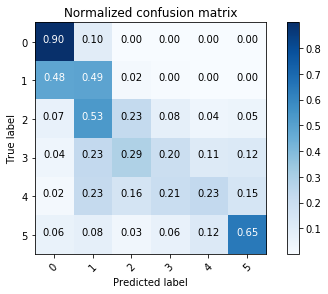
\includegraphics[width = 2.5in]{reg_clas_test}} &
\subfloat[Test]{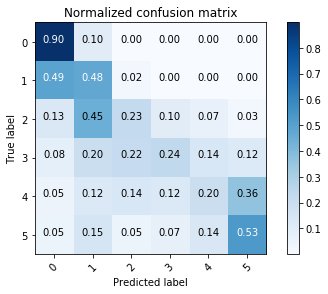
\includegraphics[width = 2.5in]{reg_clas_val}}
\end{tabular}
\caption{Normalized confusion matrix for the predictions of the transfer learning regression model converted to Ratingen-scores for the validation and test set.}
\label{fig:comparison}
\end{figure}

When comparing the normalized confusion matrix for the validation set to c) in \autoref{fig:confusion} and the normalized confusion matrix for the test set to a) in \autoref{fig:eval}, we can see that the regression model is more accurate for the labels 0, 1 and 5 whereas the accuracy for the labels 2, 3 and 4 is lower. It also seems that there are more outliers compared to the classification model, for example observations with the true label 5 that are mistakenly predicted as label 1.

\begin{table}[ht!]
\centering
\caption{Evaluation metrics for the predictions of the transfer learning regression model converted to Ratingen-scores. The normalized accuracy is the mean of the six class accuracies. Normalized $\pm$ 1 accuracy is the normalized accuracy of predictions that are in the right class or one class above or below the correct class.}
\label{tab:comparison}
\begin{tabular}{@{}lll@{}}
\toprule
                                & Validation    & Test      \\ \midrule
Accuracy					    & 0.762 & 0.754  \\
Normalized accuracy       & 0.449 & 0.429 \\
Normalized  $\pm$ 1 accuracy & 0.799 & 0.788  \\

\bottomrule
\end{tabular}
\end{table}

The evaluation metrics are compared to c) in \autoref{tab:metrics_cla} for the validation set and a) in \autoref{tab:eval_metrics} for the test set. For both the validation and the test set the accuracy of the regression model is higher, since the overrepresented class 1 is predicted very accurately. The class normalized accuracies are slightly lower than for the classification model.

\FloatBarrier

\subsection{Attention maps}
\label{subsec:attention}

In order to see where the attention of the models lie, the outputs of intermediate convolutional layers were visualized. Ideally, the last convolutional layer of the model should be visualized. However, the last convolutional layer in our classification model has the dimensions 4 x 4 which is a very low resolution and would lead to a very coarse attention map. Therefore the last convolutional layer with a dimension of 18 x 18 was chosen. In the transfer learning regression model, a similar resolution was desired. But the outputs of the last convolutional layer with the dimension 16 x 16 showed no centralized attention. Therefore we had to use a convolutional layer closer to the end of the model. The last convolutional layer with dimension 7 x 7 led to a centralized attention.

The outputs of every filter of the chosen convolutional layer were added together and normalized to values in the range [0, 1]. It was then transformed into a colormap and overlaid onto the original image. Yellow shows high attention whereas purple shows low attention.

\autoref{fig:attention} shows that the attention of both models focuses on the bone surface inside the joint and the gap between the two bones. There are a few outliers but most of the time the attention is at the correct place. This is what was desired, since the bone erosion happens in that area.

\begin{figure}[ht!]
\begin{tabular}{cc}
\subfloat[Classification]{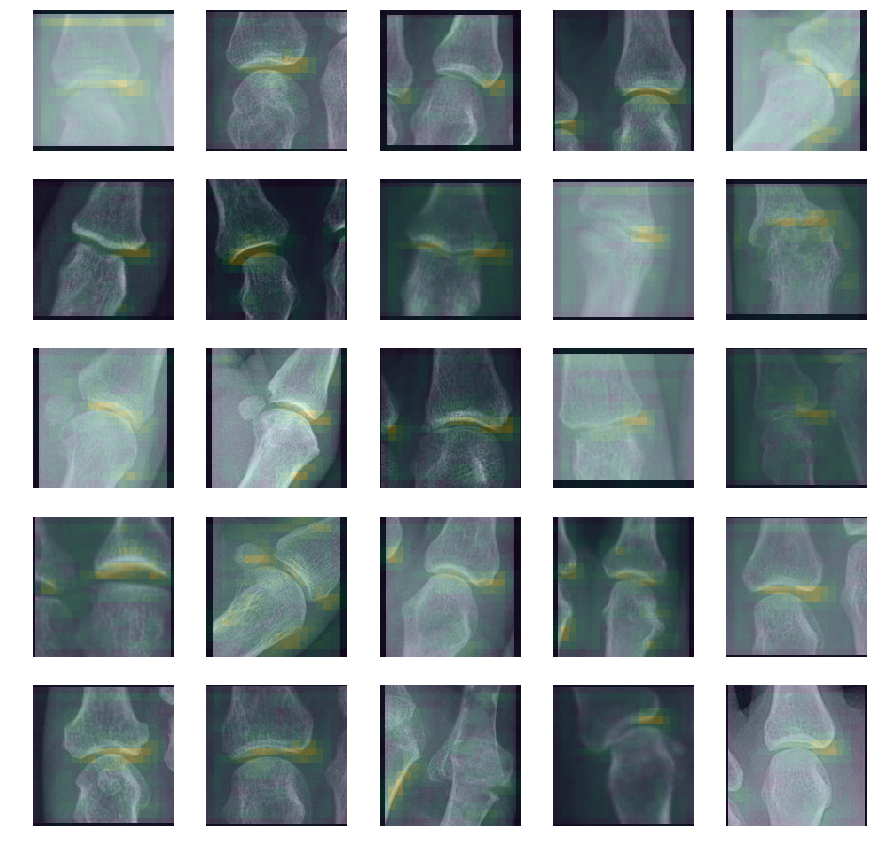
\includegraphics[width = 2.5in]{clas_attention}} &
\subfloat[Regression]{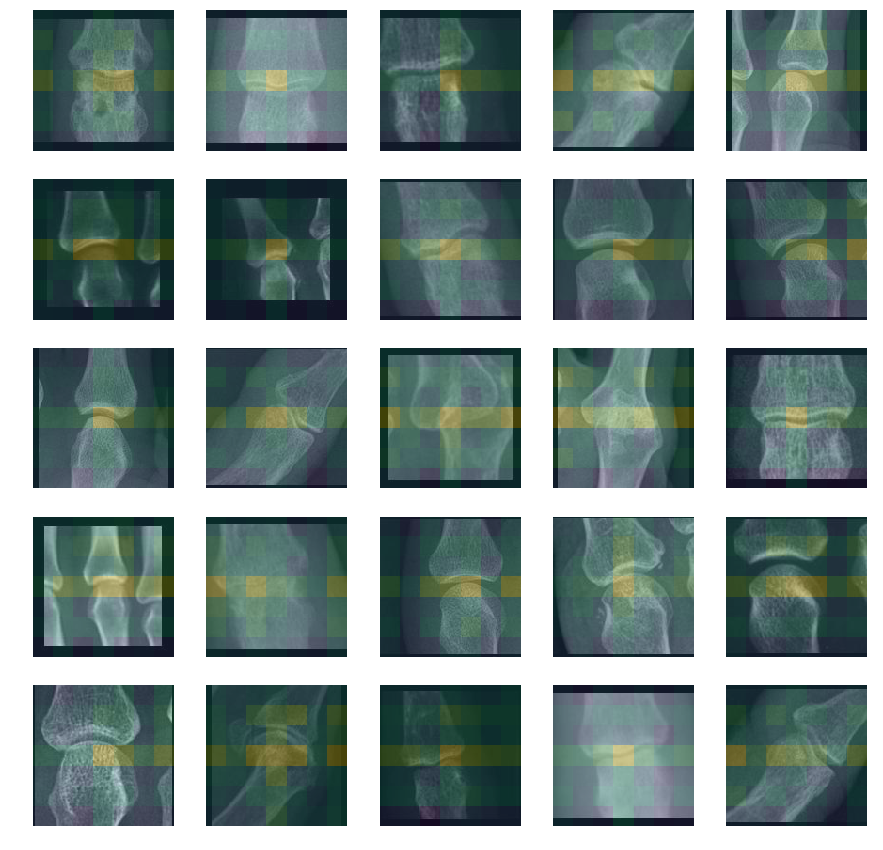
\includegraphics[width = 2.5in]{reg_attention}}
\end{tabular}
\caption{Attention maps of the best two models for random samples of the validation set. Yellow shows a high attention, whereas purple shows low attention. Most of the time the attention lies on the bone surface inside the joint.}
\label{fig:attention}
\end{figure}

\FloatBarrier

\subsection{Analysis of the embeddings}
\label{subsec:embeddings}

To visualize the high-level representations learned by our networks, t-SNE was applied to the outputs of the last hidden layer. Each dot represents an image and the colors represent the true labels of those images. \autoref{fig:tsne_embeddings} shows that both neural networks managed to separate the different scores quite well. However, there are a few images with low scores in the area of the bad scores.

\begin{figure}[ht]
\begin{tabular}{cc}
\subfloat[Classification]{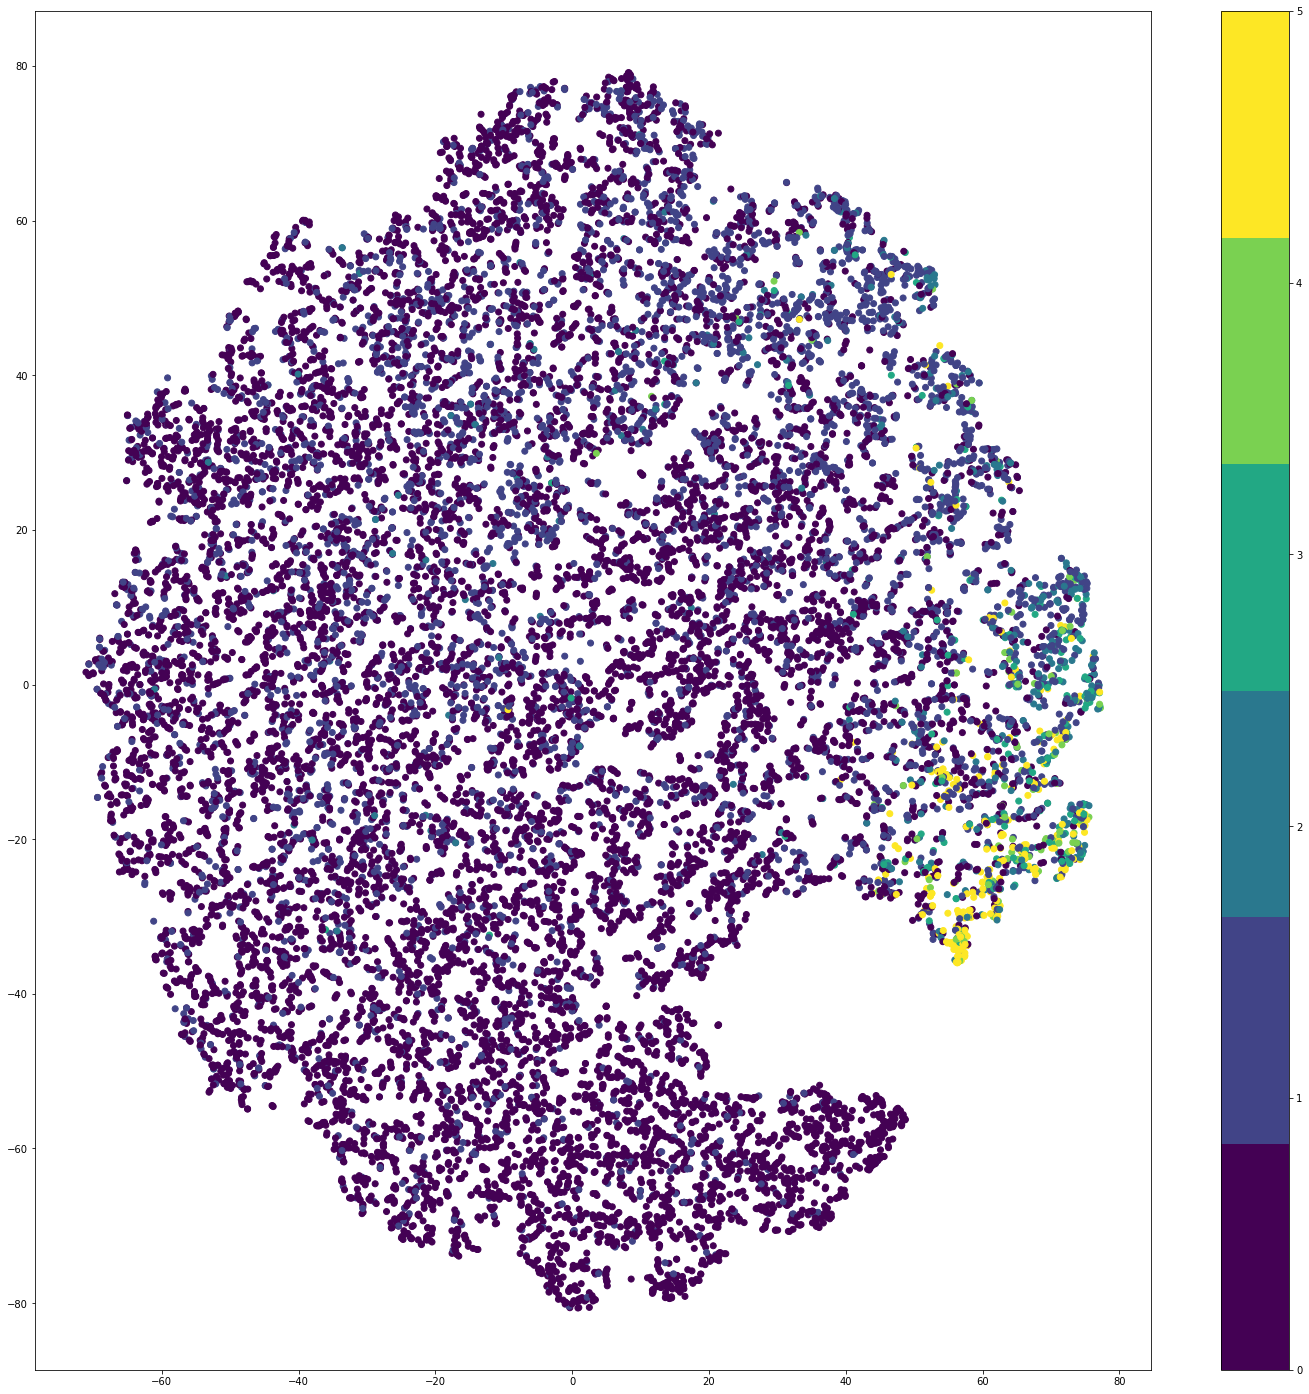
\includegraphics[width = 2.5in]{tsne_classification}} &
\subfloat[Regression]{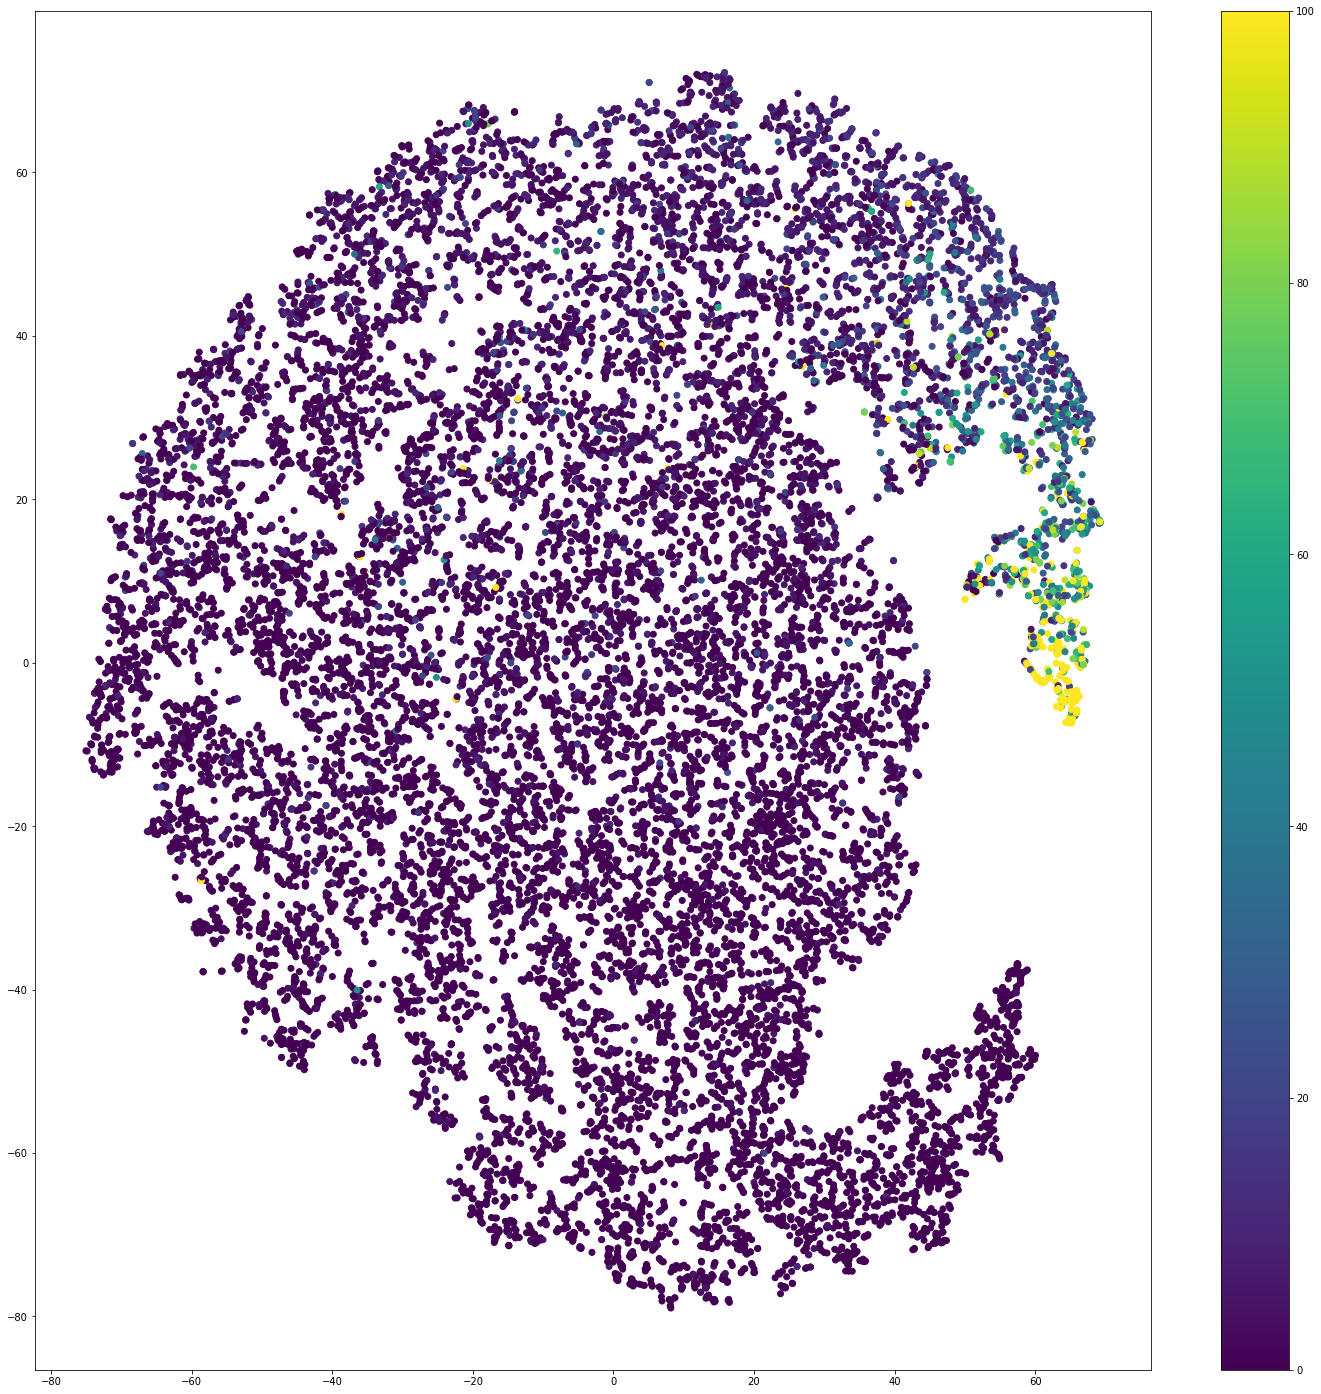
\includegraphics[width = 2.5in]{tsne_regression}}
\end{tabular}
\caption{T-SNE of the embeddings. Each point represents an image of a joint, the color represents the bone erosion score. Yellow stands for an eroded joint with a Ratingen-score of 5 or a bone erosion of 100 \%, whereas purple stands for a healthy joint with a Ratingen-score of 0 or a bone erosion of 0 \%.}
\label{fig:tsne_embeddings}
\end{figure}

Visually, it appears like the separation between the different classes is a bit more distinct in the regression model. 

\subsubsection{K-nearest-neighbors of embeddings}
\label{subsubsec:knn_embeddings}

By doing a k-nearest-neighbor (KNN) classification on the embeddings of the base classification model we can see how well the model separates the different classes. The KNN classification achieved a normalized accuracy of 31 \% which is worse than the 42 \% normalized accuracy achieved by the fully connected layers of the CNN. And also the normalized $\pm$ 1 accuracy is worse with 63 \% compared to 82 \%.

The same KNN classification was made for the embeddings of the transfer learning classification model. It achieved a normalized accuracy of 40 \% and a normalized $\pm$ of 73 \%. Both metrics are better for the embeddings of the transfer learning model than the metrics for the embeddings of the base model. This would suggest, that the transfer learning model better separates the different classes. However, a look at the confusion matrix revealed that the higher normalized accuracies are only achieved due to high accuracies for the labels 0, 1 and 5, whereas the accuracies for the labels 2, 3 and 4 are very low. This leads to the same conclusions that we made before. If the model should be a good predictor for every class, the base classification model is better suited than the transfer learning classification model.

The same analysis can be done with a KNN regression for the embeddings of the transfer learning regression model. Surprisingly, the KNN regression performs similarly well as the fully connected layers of the CNN. The MAE is a bit worse with 3.24 compared to 3.12, but the MSE is even better with 68.1 compared to 72.8. This means that instead of the fully connected layers at the end of the model also a KNN regression model could be used to make the predictions.

Again, these results are compared to the embeddings of the base regression model. The KNN regression for the embeddings of the base regression model achieved a MAE of 3.67 and a MSE of 79.1. Both scores are worse than the scores for the transfer learning model. These results support our decision to select the transfer learning regression model over the base regression model. The transfer learning model seems to better separate the different classes.

\subsubsection{Analysis of outliers in the embeddings}
\label{subsubsec:outliers_embeddings}

Next we analyzed the outliers in the embeddings of the regression model. We defined the area on the right side with majoritarian scores higher than 20 \% as the "bad area" whereas the area on the left side with majoritarian scores equal to 0 \% is called the "good area". Our hypothesis is, that the rheumatologist is more likely to score a damaged joint lower if the other joints of this patient are healthy. The same reasoning can be applied in the reverse. The rheumatologist might be more likely to give a healthy joint a higher score if the other joints of this patient are damaged.

We defined all joints with a score $\leq$ 20 \% as healthy and all joints with a score $>$ 20 \% as damaged. In the "bad area" all healthy joints are seen as outliers whereas in the "good area" all damaged joints are seen as outliers. \autoref{fig:outlier_embeddings} shows the mean scores of patients which have a joint that is an outlier in that area compared to the mean scores of patients which have a joint that is not an outlier in that area.

\begin{figure}[ht]
\begin{tabular}{cc}
\subfloat[Bad area]{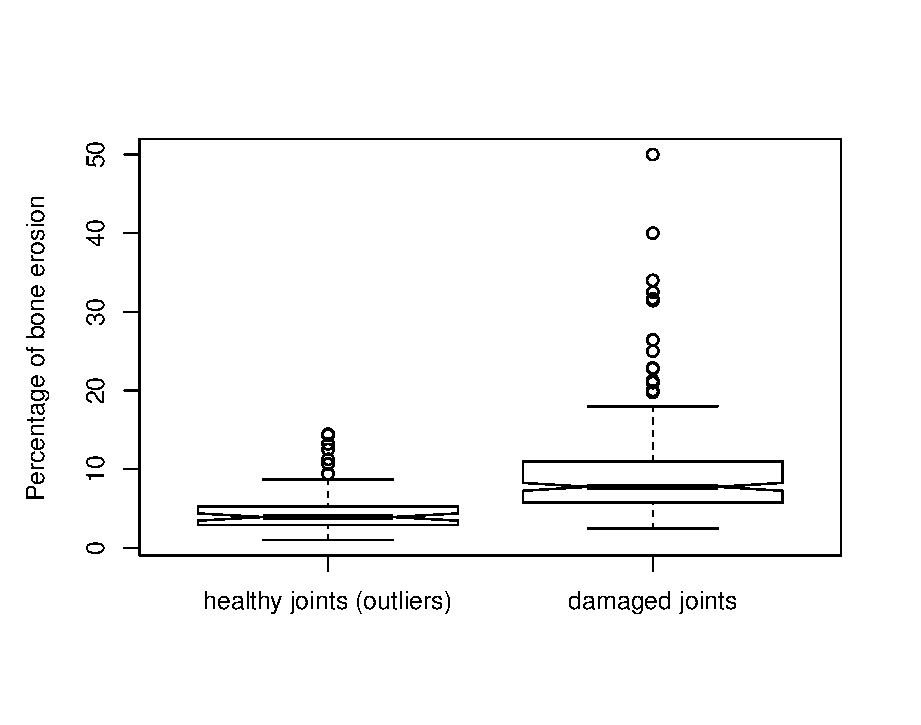
\includegraphics[width = 2.5in]{outlier_bad}} &
\subfloat[Good area]{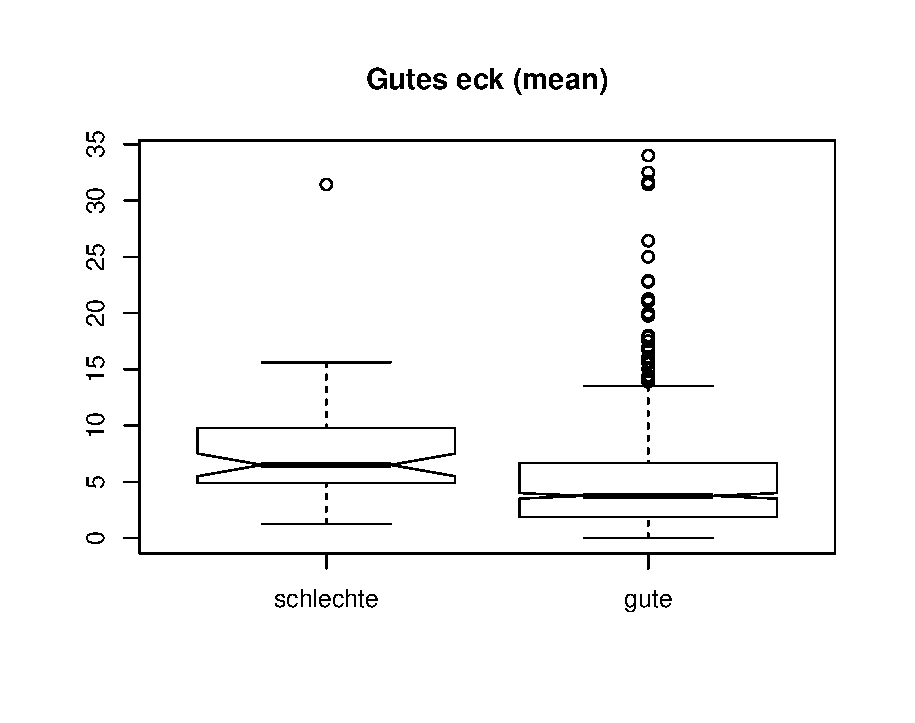
\includegraphics[width = 2.5in]{outlier_good}}
\end{tabular}
\caption{Average scores of patients which have a joint that is an outlier in that area compared to the average scores of patients that have a joint in that area which is not an outlier.}
\label{fig:outlier_embeddings}
\end{figure}

These findings support our hypothesis. Indeed outliers in the "bad area" seem to be of patients with healthier joints compared to the other patients. The opposite is true for the "good area" as well.

\FloatBarrier

\subsection{Analysis of correlations between bone erosion and disease activity}
\label{subsec:correlation}

In order to determine wether there is a correlation between the bone erosion scores and the disease activity we compared the Rau-score and the DAS. Both scores are described in \autoref{sec:theory}. It is expected that the disease activity score is correlated with the bone erosion score. However, \autoref{fig:correlation} shows that there is only a very weak correlation of 0.15 between the DAS 28 ESR and the Rau-score. The correlation between the DAS 28 CRP and the Rau-score is even weaker with 0.08.

\begin{figure}[ht!]
\begin{tabular}{cc}
\subfloat[ESR]{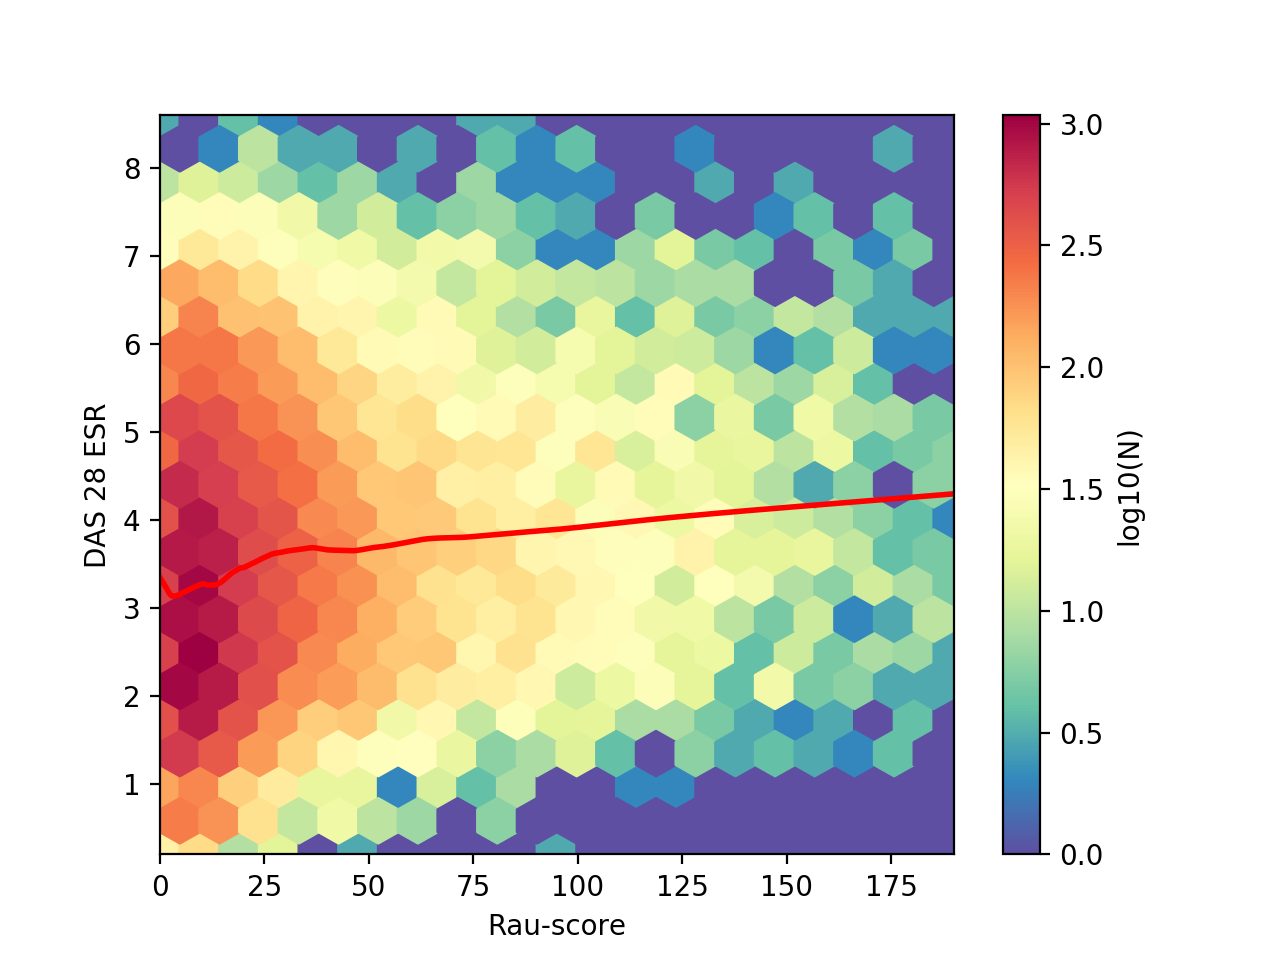
\includegraphics[width = 2.5in]{correlation_esr}} &
\subfloat[CRP]{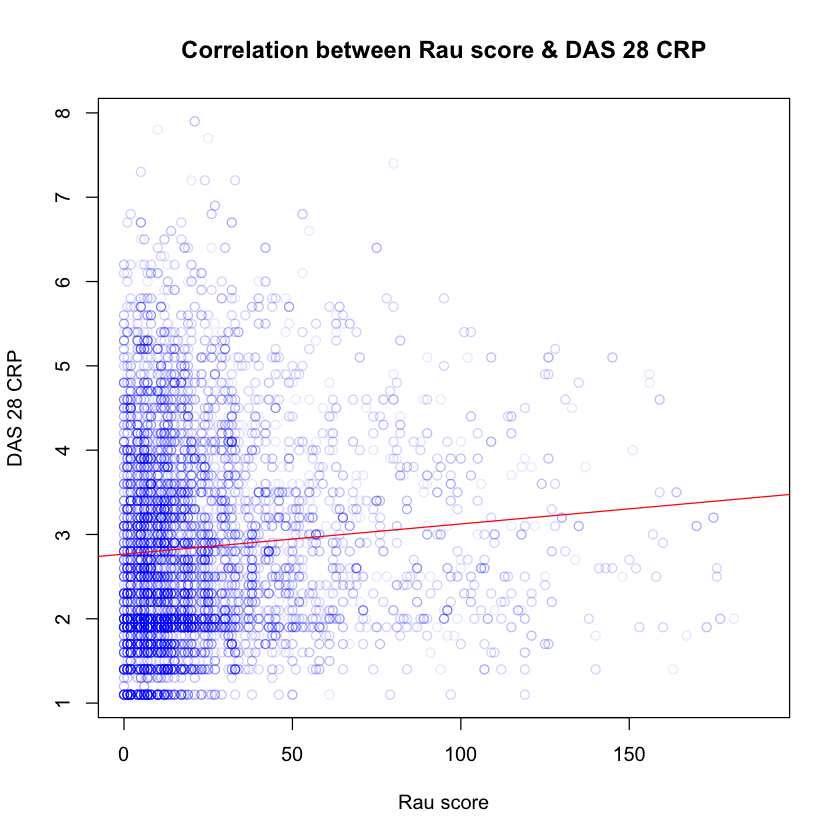
\includegraphics[width = 2.5in]{correlation_crp}}
\end{tabular}
\caption{2D histogram showing the relation between the Rau-score and the DAS score. The red line is a fitted LOESS curve. There is a small positive correlation between the DAS 28 ESR and the Rau-score. There is almost no correlation between the DAS 28 CRP and the Rau-score.}
\label{fig:correlation}
\end{figure}

This surprising result suggests that the amount of bone erosion is only a minor factor in the disease activity. 

\newpage
\section{Discussion}
\label{sec:discussion}


In the previous sections two good models were found. One for classification and one for regression. When transforming the predictions of the regression model into classes, the normalized accuracies of the two models are almost equal. However, the predictions are very differently distributed. The classification model performs similarly well for all classes whereas the regression model performs clearly better for the extreme classes 0, 1 and 5. 

It is difficult to choose one model over the other. The classification model would be better suited if a better accuracy for the intermediate classes 2, 3 and 4 is desired, whereas the regression model is better suited if accurate predictions of the extreme classes 0, 1 and 5 is desired.

An analysis of the outliers in the T-SNE shows, that there might have been a bias when the images were scored. It seems that if a patient has many damaged joints, a healthy joint is more likely to get a worse score. The opposite is true as well.

In the last section we found, that there is only a minor correlation between the percentage of bone erosion and the disease activity. While the bone erosion measures the physical damage to the joint, the disease activity score measures how much the patient suffers from the disease. Given bone erosion scores, it is almost impossible to draw conclusions regarding the disease activity.



\newpage
\section{Conclusion and outlook}
\label{sec:conclusion}

The predictions of the classification model give a good estimate for the Ratingen-score and the predictions of the regression model give a good estimate for the percentage of bone erosion. But the models are not as good as a trained professional. Many predictions are off by one Ratingen class, which corresponds to 20 \% of bone erosion. Occasional outliers are as far off as 100 \%, meaning that completely eroded joints are mistakenly classified as healthy joints or reverse. It is unclear whether an automation of the scoring process with these models can save time, since the rheumatologist still has to take a second look at the results in order to find misclassifications.

Further research could examine whether the certainty for predictions is a good indicator for outliers. In that case, the rheumatologist would only have to look at cases, where the model wasn't certain.

The attention maps showed us that the model seemed to focus on the desired part of the image. A more sophisticated approach to detect which parts of the image are responsible for the predictions, would be occluding parts of the image. A black rectangle is slided over the image do occlude different parts. For every position of the black rectangle a probability for the correct prediction can be calculated and shown as a heatmap.

Since the bone erosion scores and the disease activity are only slightly correlated, it would be interesting to examine whether the disease activity could be predicted from the images. For this task, only a slight modification to our models is necessary. One could use the classification model and change its input layer depth to 10. Instead of color channels, every channel would hold an image of a different joint from one hand.

In addition it should be investigated how different loss functions change the distribution of the predictions. For example the output layer of the regression model could be changed to only one node and the CRPS loss function could be replaced with the MSE loss function.
 

\newpage
\printbibliography

\newpage
\listoffigures

\newpage
\listoftables

\end{document}
